\documentclass{article}
\usepackage{icml2017}

\usepackage{graphicx}

\usepackage{amsmath}
\usepackage{amsthm}
\usepackage{amssymb,latexsym,color}
\usepackage{mdwlist}
\usepackage{todonotes}
%\usepackage{fullpage}
%\usepackage{charter}

\usepackage{url}

\usepackage{wrapfig}

%\usepackage{algorithm}
%\usepackage[noend]{algpseudocode}

%\usepackage{fullpage}
\usepackage{marvosym}
%\usepackage[techreport]{systems-cover}
\usepackage{natbib}
\usepackage{graphicx}
\graphicspath{ {Figures/} }
\usepackage{subcaption}
%\captionsetup[subfigure]{justification=justified,singlelinecheck=false}

\newcommand{\R}{\mathsf{R}}
\newcommand{\sgn}[1]{\mbox{sgn}(#1)}
\renewcommand{\vec}[1]{\mathbf{#1}}

\def\a{{\bf a}}
\def\g{{\bf g}}
\def\x{{\bf x}}
\def\y{{\bf y}}
\def\w{{\bf w}}
\def\v{{\bf v}}
\def\E{\mathbb{E}}
\def\rrow{r_\mathrm{row}}

\def\Ji{Ji's comment}

\DeclareMathOperator*{\argmin}{argmin}

\newtheorem{lemma}{Lemma}
\newtheorem{theorem}{Theorem}
\newtheorem{claim}{Claim}
\newtheorem{corollary}{Corollary}
\newtheorem{prop}{Proposition}
\newtheorem{definition}{Definition}

%\newcommand{\todo}[1]{\noindent \textbf{[TODO:] #1 } }
\usepackage{mathtools}
\DeclarePairedDelimiter\floor{\lfloor}{\rfloor}
\DeclarePairedDelimiter\ceil{\lceil}{\rceil}

\date{}

%\title{Training Generalized Linear Models with End-to-end Low Precision:\\
%The Cans, the Cannots, and a Little Bit of Deep Learning
%}
\title{Training with End-to-end Low Precision:\\
The Cans, the Cannots, and a Little Bit of Deep Learning
}


\begin{document}
\maketitle

\begin{abstract}

There has recently been significant interest in training 
machine-learning models at low precision: by reducing 
precision, one can reduce computation, communication, and power 
consumption by one order of magnitude. 
We examine this from a theoretical and practical 
perspective. We ask: 
{\em is it possible to \emph{train} models at end-to-end low 
precision with \emph{provable} guarantees?  can this 
lead to consistent order-of-magnitude speedups?}

For linear models, the answer is yes. We develop a simple 
framework based on one novel strategy: ``double sampling''. 
With our framework, it is able 
to execute training at low precision with no bias, 
guaranteeing convergence, while naive stochastic quantization 
would introduce significant bias. We validate this  
across a range of applications, and show that it enables an 
FPGA prototype that is up to one order of magnitude faster 
than an implementation using full 32-bits precision.

We extend our framework through approximation to non-linear 
models, such as SVM. We show that, although the bias of using 
low precision data cannot be avoided, our approach can appropriately 
control the bias. We find that in practice {\em 8-bits} precision is 
always sufficient to converge to the correct solution. 
Interestingly, however, in practice, we notice that our framework 
does not always outperform the naive rounding approach. We discuss 
this negative result in detail. 

Further, we develop a variance-optimal 
stochastic quantization
strategy and show that 
it can make a significant difference in a variety of settings. 
When applied to linear models together with 
double sampling, we can save up to another 
$2\times$ communications
compared with uniform quantization. When
training deep networks with quantized models, 
we achieve higher accuracy than state-of-the-art XNOR-Net. 

\end{abstract}

\begin{figure}[t]
\centering
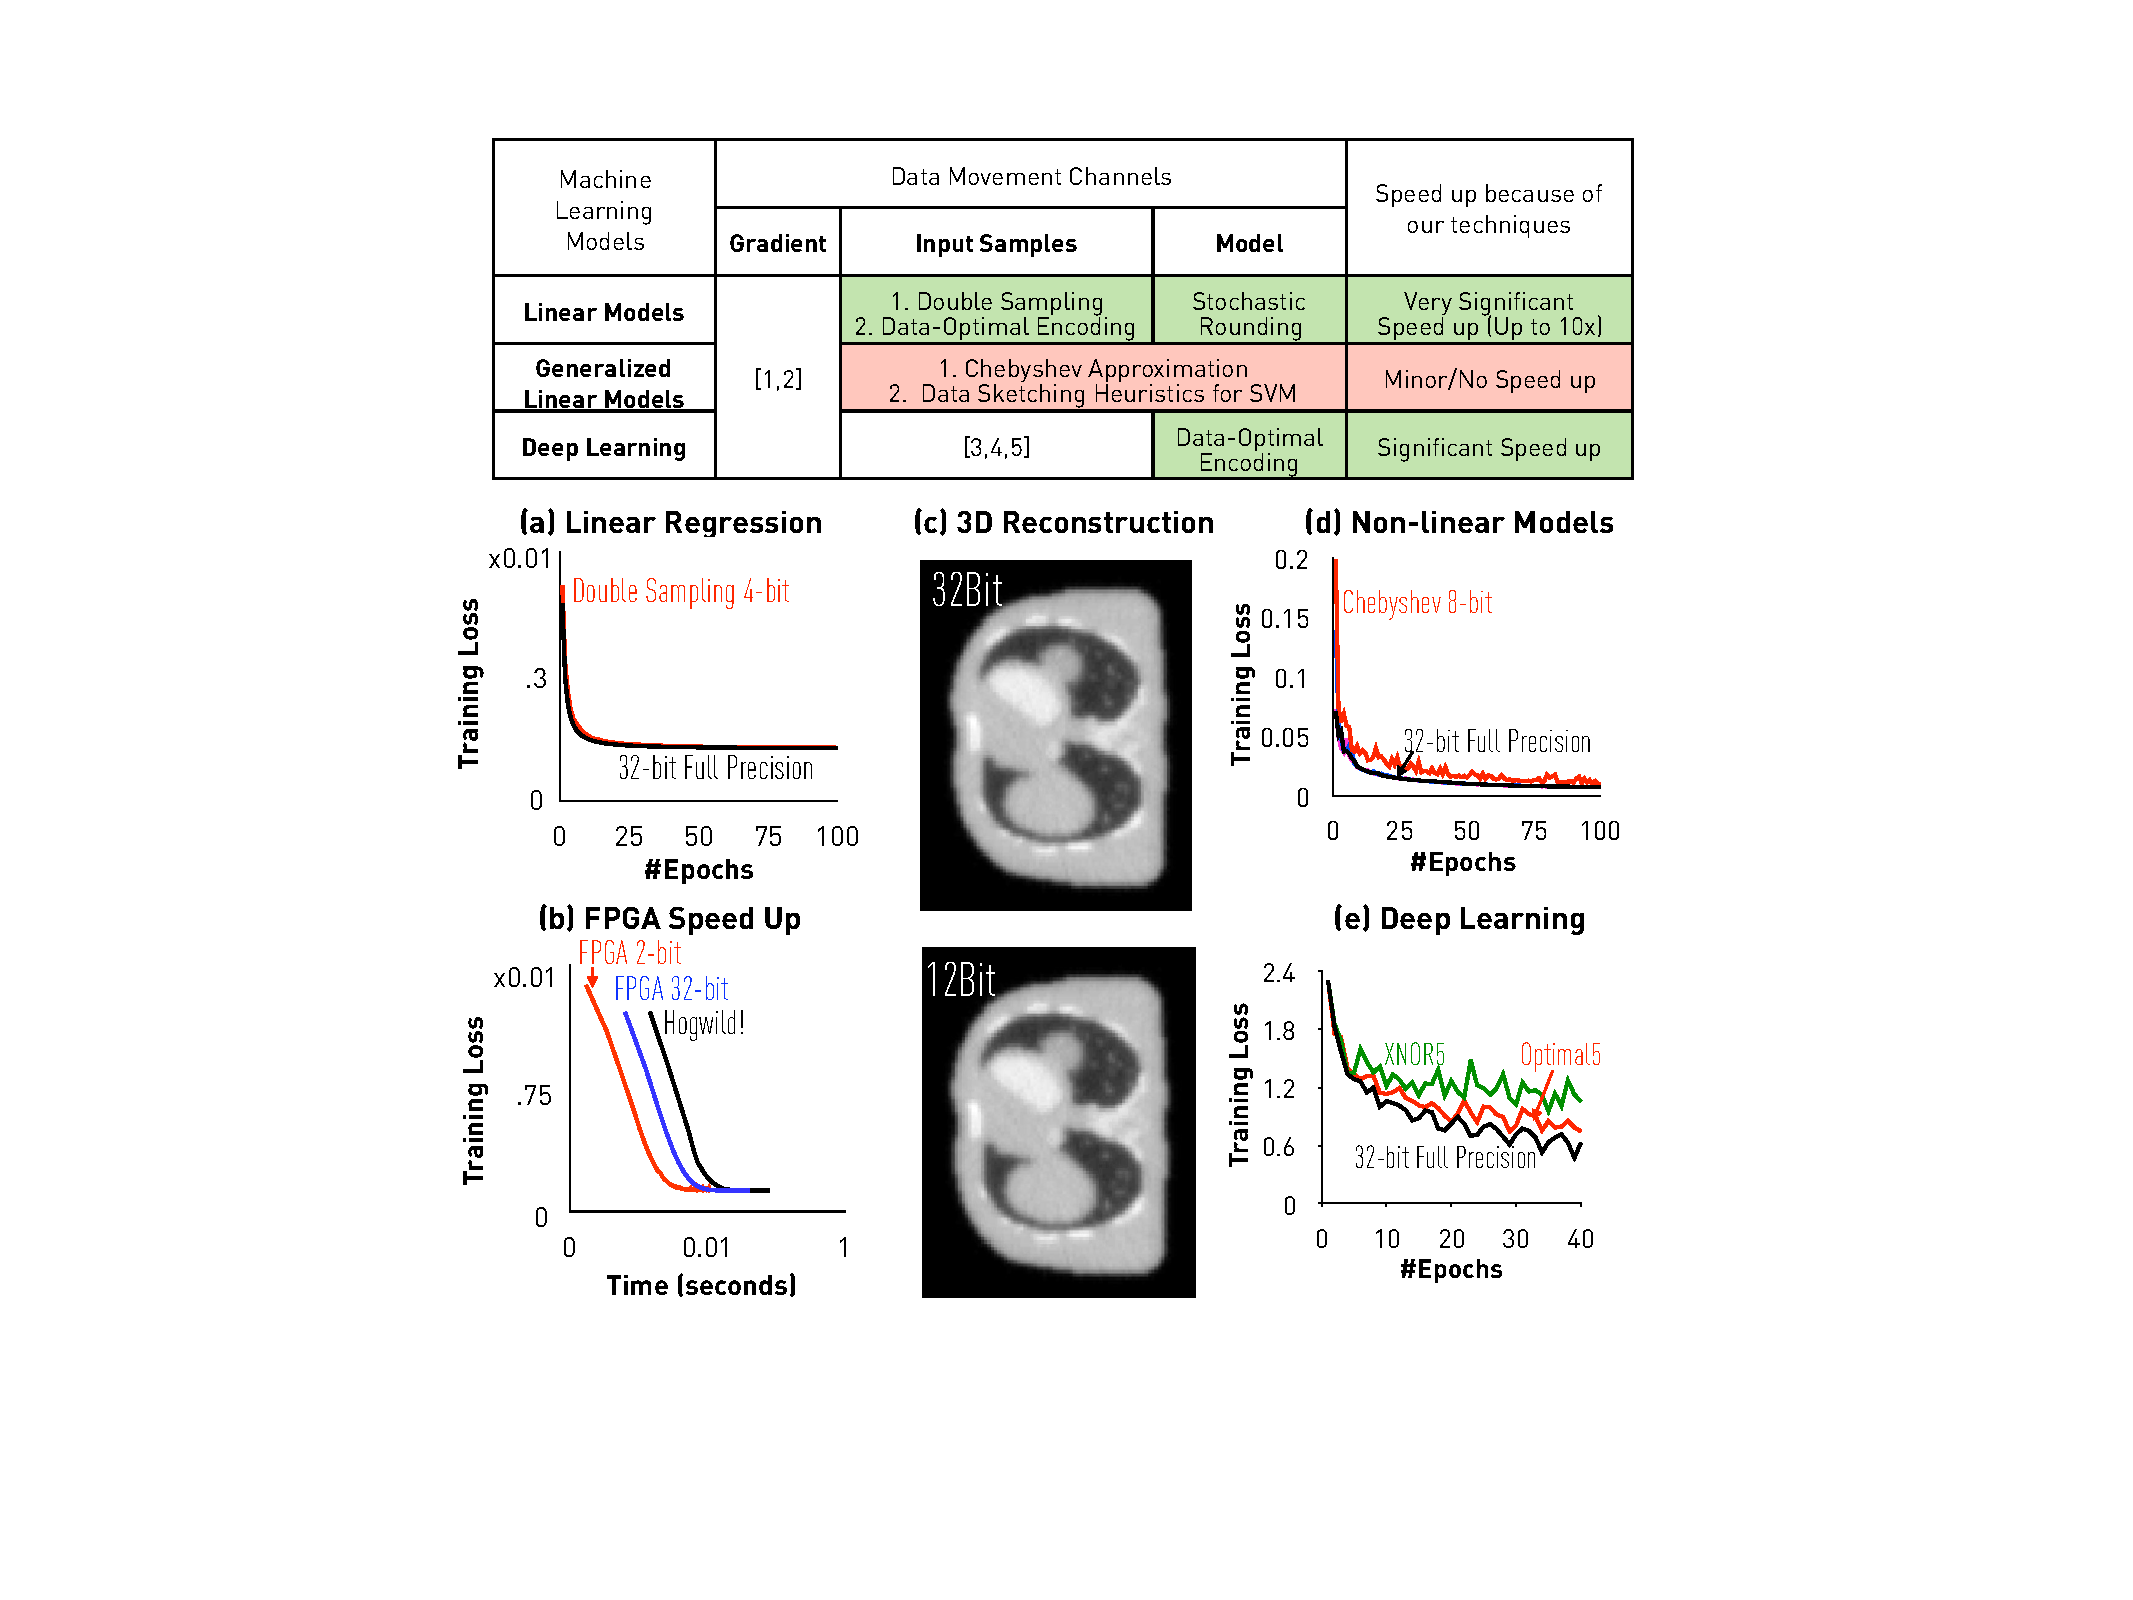
\includegraphics[width=0.5\textwidth]{Figures/RSHighlight}    
\vspace{-2em}
\caption{Overview of theoretical results and
highlights of empirical results. See
Introduction for details.}
\label{fig:highlight}
\end{figure}
\vspace{-2em}
\section{Introduction}

The computational cost and power consumption of today's machine learning systems are often driven by data movement, and by the precision of computation. 
In our experience, in applications such as tomographic reconstruction, anomaly detection in mobile sensor networks, or compressive sensing, the overhead of transmitting the data samples can be massive, 
and hence performance can hinge on reducing the precision of data representation and 
associated computation. 
A similar trend is observed in deep learning, where impressive progress has been reported with systems 
using end-to-end reduced-precision representations~\cite{hubara2016quantized,
rastegari2016xnor,zhou2016dorefa,miyashita2016convolutional}. 
In this context, the motivating question behind our work is:  {\em When training general machine learning models,
can we lower the precision of data representation,
communication, and computation, while maintaining provable guarantees?}
 
% 
%The total operating costs
%or power consumptions of 
%today's machine learning systems 
%are often bounded by data 
%movement and precision of computation.
%From our experience in supporting
%multiple industry partners with 
%a diverse set of applications
%such as tomographic reconstruction,
%anomaly detection over mobile 
%sensor networks, compressive sensing,
%or Ridge regression over
%enterprise data, many of these 
%applications hinge on one question: {\em
%When training generalized linear models,
%can we lower the precision of data representation,
%communication, and computation?}
%
%On the other hand, the Deep Learning
%community has recently witnessed a
%tremendous success in  
%end-to-end low-precision, sometimes as
%low as a single bit, training of neural networks
%with negligible quality loss in many cases~\cite{XXX,XXX,XXX,XXX,
%XXX,XXX,XXX,XXX,XXX}. {\em Can we apply
%these techniques to simpler generalized
%linear models?}

In this paper, we develop a general 
framework to answer this question, and
present both  positive and negative results
 obtained in the context of this framework. 
 Figure~\ref{fig:highlight} encapsulates our results: 
(a) for linear models, we are able to lower the precision of both computation and communication, including input samples, gradients, and model, by up to $16$ times, while still providing rigorous theoretical guarantees; 
(b) our FPGA implementation of this framework achieves up to $10\times$ speedup compared with
a 32-bit FPGA implementation, or with a 10-cores CPU running Hogwild!;  
(c) we are able to decrease data movement by $3\times$ for
tomographic reconstruction, while getting negligible quality decrease. 
Elements of our framework generalize to (d) non-linear models and  (e) model compression for training deep learning models. 
In the following, we describe our technical contributions in more detail. 


%In this paper, we develop a general 
%framework to answer these questions, and
%present both the positive and negative results
%we obtained. Figure~\ref{fig:highlight} encapsulates our results: 
%(a) for linear
%models, we are able to lower the precision of computation and communication, including input samples, gradients, and model, by up to $16$ times, while still providing rigorous theoretical guarantees 
%we are able to lower the precision of all
%computation and communication involving
%input samples, gradients, and models, by up to 
%$16\times$; (b) when implemented on FPGA, we achieve
%up to $10\times$ speed up compared with
%a 32-bit FPGA implementation and a 10 cores
%CPU running Hogwild!; and (c) we are able to
%decreases data movement by 3$\times$ for
%tomographic reconstruction while getting
%innegligible quality decrease. Our framework
%also applies to (d) non-linear models and 
%(e) model compression for training deep
%learning models. We now summarize our
%technical contributions.


\subsection*{Summary of Technical Contributions}

We first consider the following problem in training generialized linear models: 
\begin{align}
\min_{\x}:\quad {1\over 2K}\sum_{k=1}^K l(\a_k^\top \x, b_k)^2 + R(\x)
\label{eqn:leastsquares}
\end{align}
where $l(\cdot,\cdot)$ is a loss function, and $R$ is a regularization term, which could be $\ell_1$ norm, $\ell_2$ norm, or even an indicator function representing the constraint. 
The gradient at the sample $(\a_k, b_k)$ is: 
\[
\g_k := \a_k \frac{\partial l(\a_k^\top \x, b_k)}{\partial \a_k^\top \x} 
\]
We denote the problem dimension by $n$. 
We consider the properties of the algorithm when a lossy compression scheme is applied to the data (samples), 
gradient, and model, for the purpose of reducing the communication cost of the algorithm---That is, 
we consider $Q_1$, $Q_2$, and $Q_3$ in the gradient update rule:
\begin{align}
\x_{t + 1} \leftarrow \text{prox}_{\gamma R(\cdot)}\left(\x_t - \gamma Q_1(\g_k (Q_2(\x_t), Q_3(\vec{a}_t)))\right).
\label{eq:proxupdate}
\end{align}
where the proximal operator is defined as
\[
\text{prox}_{\gamma R(\cdot)}(\y) =\argmin_{\x} {1\over 2}\|\x-\y\|^2 + \gamma R(\x).
\]

\subsection{Our Results}

We summarize our results as follows. The {\bf (+)}
sign means ``positive result'' where we achieve
significant practical speedup, and {\bf (--)} otherwise.

\paragraph{(+) Linear Models.} When $l(\cdot,\cdot)$ is 
the least squares loss, we first prove that
simply doing stochastic quantization of data 
(i.e., $Q_3$) introduces bias of the gradient
estimator and therefore SGD would converge
to a different solution. We propose a simple
fix to this problem by introducing a
{\em double sampled} quantization strategy
$\tilde{Q}_3$ that uses multiple samples to
eliminate the correlation of samples introduced
by the non-linearity of the gradient. We
analyze the additional variance introduced
by double sampling, we find \textcolor{red}{
BLAH BLAH BLAH BLAH BLAH BLAH BLAH BLAH BLAH BLAH BLAH BLAH
BLAH BLAH BLAH BLAH BLAH BLAH}. Using
stochastic quantization for gradient and model,
this gives us an end-to-end quantization strategy
for linear models, whose variance is \textcolor{red}{
BLAH BLAH BLAH BLAH}.

\vspace{-1em}
\paragraph{(--) Non-Linear Models.} We extend our
results to non-linear models such as
logistic regression and SVM. We observe that
using multiple samples can, in principle,
provide unbiased estimators for any polynomials
(with an increased variance). Our main
result uses Chebyshev polynomials to
approximate the gradient and provide theoretical
bound on the bias introduced by Chebyshev
approximation and the bias of SGD solution. 
This provides a way to control the bias given
users' error tolerance as input.  
When data is separable,
we prove that \textcolor{red}{BLAH BLAH 
BLAH BLAH BLAH BLAH BLAH BLAH BLAH BLAH BLAH 
BLAH BLAH BLAH}. With this technique, we are
able to lower the precision by 4$\times$ with
rigorous theoretical guarantee; However,
compared with a strawman approach that just
do stochastic rounding over input data, 
\textcolor{red}{BLAH BLAH BLAH BLAH.}.

\vspace{-1em}
\paragraph{(+) Optimal Quantization and Extension to Deep Learning.}
We then focus on variance reduction for 
stochastic quantization. We observe that different
quantization points have different variances---the points chosen
by standard fixed point representation is uniformly
distributed but is not optimal.
We formulate an optimization problem to choose 
quantization points that minimize the total variance
introduced by quantization and solve it with 
a dynamic programming algorithm with time complexity
$O(BLAH)$ and space complexity $O(BLAH)$.
When applied to linear models, this optimal 
strategy can save up to $2\times$ communication
compared with the uniform strategy.

Our analysis of optimal quantization 
implies that the uniform quantization approach
popularly used by state-of-the-art end-to-end
low-precision deep learning training systems
when more than 1 bit is used are also suboptimal.
We then apply optimal quantization to 
model quantization and shows that, with a simple
standard neural network, we outperforms the
uniform quantization used by XNOR-Net and a
range of other recent approaches. This
is relevant, but slightly different, to some work 
on model compression for inference~\cite{Han:2016:ICLR}, 
but to our best knowledge, it is the first time it 
has been applied to training. 

\section{Linear Models}

\vspace{-0.5em}
In this section, we focus on linear models.
We have labeled data points $(\a_1, b_1), (\a_2, b_2), \ldots, (\a_K, b_K) \in \R^n \times \R$, and our goal is to minimize the function
\[
f(\x) = \frac{1}{K} \sum_{k = 1}^K \| \a_k^\top \x - b_k \|_2^2 \; ,
\]
i.e., minimize the empirical least squares loss.
The full-precision (unquantized) SGD works as 
follows: at step $\x_k$, our gradient estimator is $\g_k^{(full)} = \a_{\pi(k)} (\a_{\pi(k)}^\top \x - b_{\pi(k)})$, where $\pi(k)$ is a uniformly random integer from $1$ to $K$.
We abuse the notation and let $\a_k = \a_{\pi(k)}$.
It is not hard to see that $\E [\g_k^{(full)}] = \nabla f(\x_k)$.

\vspace{-1em}
\paragraph*{Quantization Function $Q$} We define
the quantization function $Q$ that we will use
for the rest of this paper. Given a vector
$\v$, let $M(\v)$ be a scaling factor such that
$-1 \le \v/M(\v) \le 1$. Without loss of generality,
let $M(\v)=||\v||_2$. We partition
the interval $[-1, 1]$ using $s+1$ separators:
$-1 = l_0 \le l_1 ... \le l_{s} = 1$; for
each number $v$ in $\v/M(\v)$, we always 
quantize it to one of two nearest 
separators: $l_i \le v \le l_{i+1}$. 
We denote the quantization function by $Q(\v, s)$
and choose the probability of quantizing to
different separators such that $\E[Q(\v, s)] = \v$.
We use $Q(\v)$ when $s$ is not relevant.
We assume that these
separators are uniformly distributed,
and revisit this in Section~\ref{sec:optimal}.

\vspace{-1em}
\subsection{Naive Stochastic Quantization is Biased}

\vspace{-0.5em}
We focus on quantizing the input samples.
We first establish that, when we quantize $\a_k$
using the stochastic quantization methods designed
for gradient, it introduces significant bias.
Let $\hat{\a_k} = Q(\a_k)$ be the quantized
sample, the gradient becomes
\[
\g_k := \hat{\a_k} \hat{\a_k}^\top \x - \hat{\a_k} b_k.
\]
It is not hard to see that the expected gradient is: 
\[
\E[\g_k] := \a_k \a_k^\top \x - \a_k b_k + D_{\a} \x, 
\]
where $D_{\a}$ is diagonal and its $i$th diagonal element is 
\[
\E[ Q(\a_i)^2 ] - \a_i^2.
\]

\begin{wrapfigure}{r}{0.23\textwidth}
  \begin{center}
    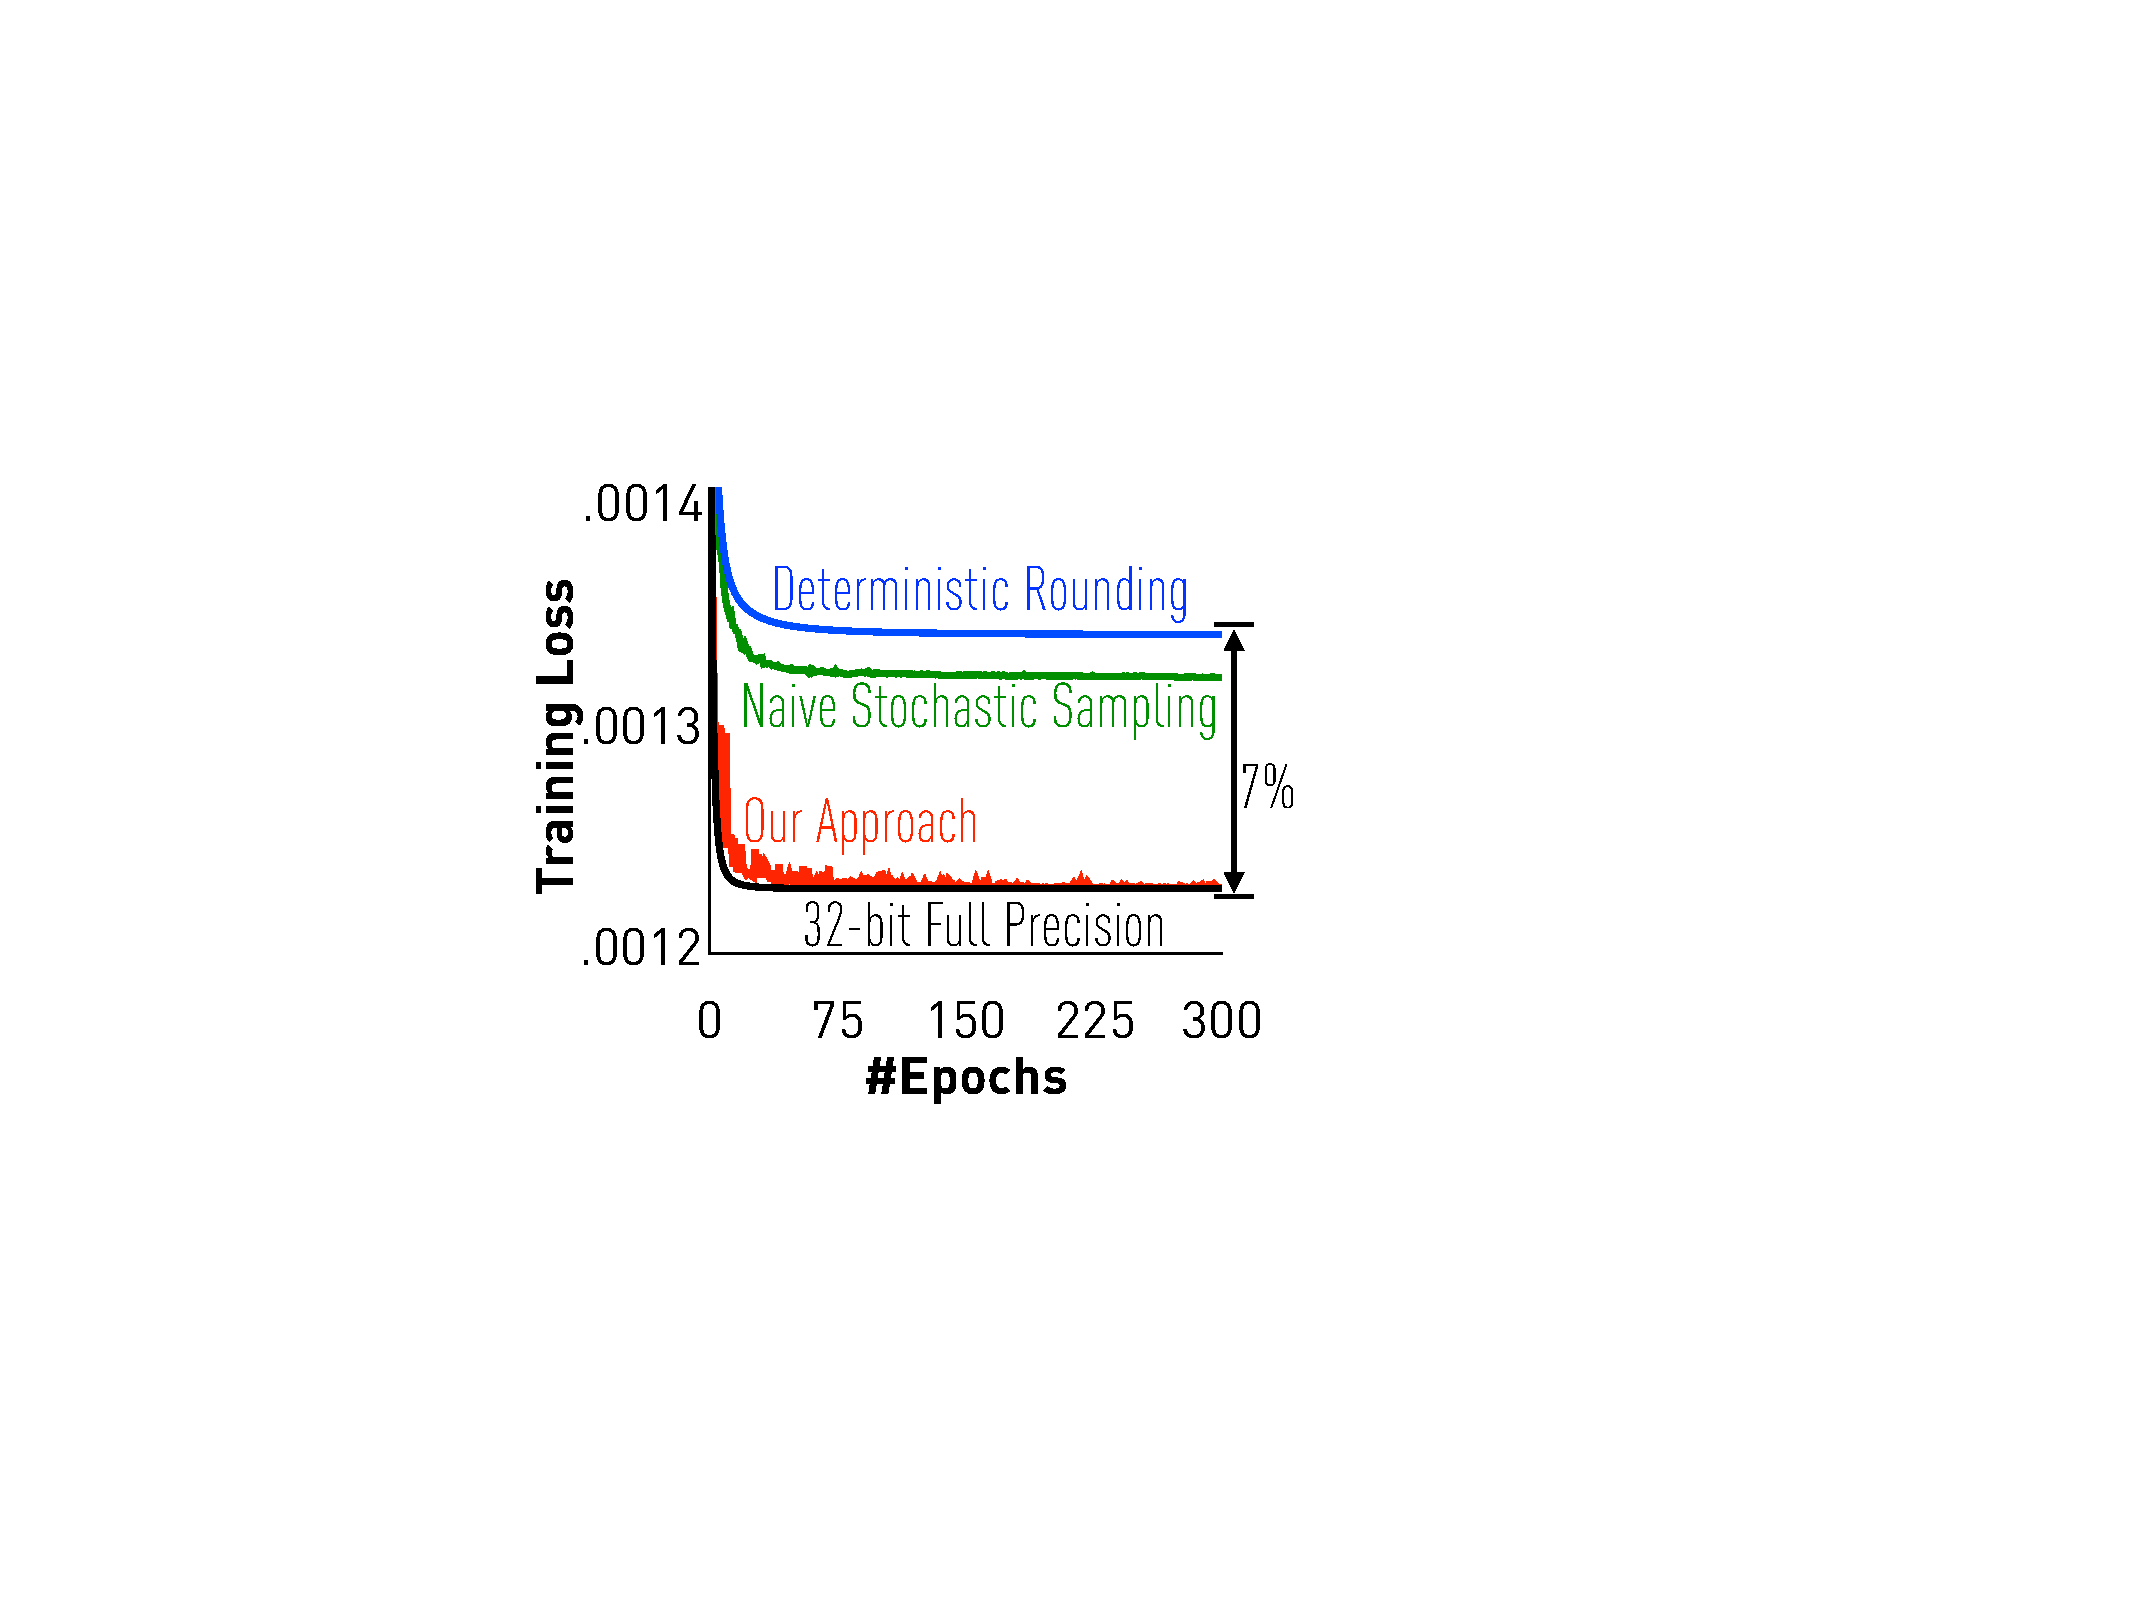
\includegraphics[width=0.23\textwidth]{micro-experiments/gap.pdf}
  \end{center}
  \label{fig:gap}
\end{wrapfigure}

Since $D_{\a}$ is non-zero, we obtain a \emph{biased} estimator of the gradient, so the iteration is unlikely to converge. 
The figure on the right illustrates the bias
caused by a non-zero $D_{\a}$.
In fact, it is easy to see that in instances where the minimizer $\x$ is large and gradients become small, we will simply diverge. 

\subsection{Double Sampling}

We now present a simple method to fix the biased gradient estimator.
We generate two independent
random quantizations and revise the gradient:
\[
\g_k := Q_1 (\a_k) (Q_2 (\a_k)^\top \x + b_k) \; .
\]
This gives us an unbiased estimator 
of the gradient.

\paragraph{Variance}

Let $r = r(s) = 1 + \min (n / s^2, \sqrt{n}/ s)$ be the blow-up in the second moment.
We have:
\begin{lemma}
\label{lem:qbound}
    Given $\a_k, \x, b_k$, suppose $\| \a_k \|_2^2 \leq A^2, \| \x \|_2^2 \leq R^2$ and $\max_i |\a_k| \leq M_a$.
    Let $\g_k^{(full)}$ be the unquantized stochastic gradient. We have
    \[
    E_{Q_1, Q_2} [\| \g_k \|_2^2] \leq r \cdot \left( \| \g_k^{(full)} \|_2^2 \cdot \frac{M_a^2}{\| \a_k \|_2^2} + \frac{A^2 M_a^2 R^2}{s^2} \right)\; .
    \]
\end{lemma}

In particular, this implies the following variance bound on our quantized updates:
\begin{corollary}
    Let $\a_k, \x, b_k, \g_k^{(full)}$ be as above.
    Suppose $\E [\| \g_k^{(full)} - \nabla f(\x_k) \|_2^2 ] \leq \sigma^2$ and $\E [\| \g_k^{(full)} \|_2^2] \leq B$. We have
    \[
    \E \left[ \| \g_k - \nabla f(\x_k) \|_2^2 \right] \leq  \sigma^2 + \left(r \frac{M_a^2}{\| \a_k \|_2^2} - 1\right) B + \frac{r A^2 M_a^2 R^2}{s^2} \; ,
    \]
    where the expectation is taken over $\g_k^{(full)}$ and the randomness of the quantization.
\end{corollary}

This corollary suggests that the quantized stochastic gradient variance is bounded by
\[
\E \left[ \| \g_k - \nabla f(\x_k) \|_2^2 \right] \leq \sigma^2 + \Theta(n/s^2) \;
\]
in the scenario when $M_i (\vec{v}) = \| \vec{v} \|_2 $.
The first term $\sigma^2$ is introduced by stochastic gradient, while the second term is introduced by quantization. Because the value of $s$ is 
exponential to the number of bits, to ensure these two terms are comparable (to maintain the same convergence rate of quantized stochastic gradient), the number of bits needs to be greater than $\Theta(\log n / \sigma)$. We see that even for linear models with millions
of features, 32-bits is likely to be an ``overkill''.

\paragraph*{Overhead of Storing Two Samples}
One system implication of double sampling is the overhead of sending
two samples instead of one. We note that this will not introduce $2\times$
overhead in terms of data communication, instead, just a single more bit
for the second sample because of the correlation between two samples (they 
are only different by at most one bit). More generally, because samples
are used symmetrically, sending $k$ samples only require $\log_2 k$ more bits.

\paragraph*{Extensions}

All of our results can be applied to 
optimization problems 
with possibly non-smooth regularization term. The key substitution is to use the proximal update defined in \eqref{eq:proxupdate}.
Also, extending our result to least-squares SVMs for classification is trivial~\cite{Suykens:1999:Book}.
We leave these details to the full version
of this paper.

\subsection{End-to-end Quantization}

We can now develop an end-to-end quantization strategy that
quantizes gradients, model, and input samples all 
at the same time. The gradient becomes:
\[
\g_k := Q_1 \left( Q_2(\a_k, s ) ( Q_3(\a_k, s)^\top Q_4(\x, s) + b_k) , s \right),
\]
\noindent 
where all $Q$'s are independent quantizations.

%  $Q_3$ and 
%The iteration becomes: 
%
%\begin{eqnarray}
%	\x = \x - \gamma \g_k.
%\end{eqnarray}

\noindent From combining the previous results, we have:

\begin{corollary}
    \label{cor:full-quantization}
    Let $\a_k, \x, b_k$ be so that $\| \a_k \|_2^2 \leq 1, \| \x \|_2^2 \leq R^2$.
    Let $M_a, M_x$ be as above, and let $\g_k^{(full)}$ be the (unquantized) stochastic gradient.
    We have
    \[
    \E [\| \g_k \|_2^2] \leq r \cdot \left( r M_a \left( \| \g_k^{(full)} \|_2^2 + \frac{R^2}{s^2} \right)  + \frac{r^2 M_a^2 R^2}{s^2} \right) \; .
    \]
\end{corollary}


%!TEX root = main.tex
\section{Non-Linear Models}

In this section, we extend our framework to approximate arbitrary classification losses within arbitrarily small bias. 
Although theoretically justified, this framework can become heavyweight for loss functions which are not well approximable by polynomials 
(e.g., hinge). We provide efficient quantization heuristics for these loss functions. 

\subsection{Quantizing Arbitrary Polynomials} 

Assume we are given a degree $d$ polynomial $P(x) = \sum_{i = 0}^{d} m_i z^i$, and that 
we wish to evaluate it at $\vec{a}^\top \vec{x}$, while quantizing $\vec{a}$, so as to preserve the value of $P( \vec{a}^\top \vec{x})$ in expectation. 
We do so as follows. 

We will use $d$ independent quantizations of $\vec{a}$, $Q_1(\vec{a}), Q_2(\vec{a}), \ldots, Q_d(\vec{a})$. 
Given these quantizations, our reconstruction of the polynomial will be 
$$ Q(P) := \sum_{i = 0}^d m_i \prod_{j \leq i} Q_j(\vec{a})^\top \vec{x}.$$

The fact that this is an unbiased estimator of $P( \vec{a}^\top \vec{x} )$ follows from the independence of the quantizations. Extending the analysis in Lemma~\ref{lem:qbound} yields:

\begin{lemma}
\label{lem:poly-sec-moment-bound}
	$\E[ Q(P)^2 ] \leq 2^d \sum_{i = 0}^d m_i r(s)^i (\vec{a}^\top \vec{x})^i.$
\end{lemma} 








\subsection{Quantizing Arbitrary Classification Losses}

Assume a standard classification setting, where we have samples $[(\vec{a}_i, b_i)]_i$ drawn from a distribution $\mathcal{D}$, a loss function $\ell: \R \rightarrow \R$, and we wish to find $\vec{x}$ which minimizes $\E_{\mathcal{D}} [ \ell( b \cdot \vec{a}^\top \vec{x} ]$. The gradient of $\ell$ is given by 
$$ \nabla_\vec{x} (b \cdot \vec{a}^\top \vec{x}) = b \ell' (b \cdot \vec{a}^\top \vec{x}) \vec{a}.$$

Assume normalized samples, i.e. $\| \vec{a}_i \|_2 \leq 1, \forall i$, and that $\vec{x}$ is constrained such that $\| \vec{x} \|_2 \leq R$, for some real value $R > 0$. We are given a target accuracy $\epsilon$, within which we wish to approximate the gradient. 

Given this, we fix the minimal-degree polynomial $P$ such that $|P(z) - \ell'(z)| \leq \epsilon, \forall z \leq R$. This polynomial is known to both transmitter (sample source) and receiver (compute device). The protocol is as follows. 
\begin{itemize}
	\item For a given sample $(\vec{a}_i, b_i)$ to be quantized, the source will transmit $b_i$, as well as $d + 1$ independent quantizations $Q_1, Q_2, \ldots, Q_{d + 1}$ of $\vec{a}_i$. 
	\item The receiver computes $b \cdot Q(P) Q_{d + 1} ( \vec{a}_i )$ and uses it as the gradient.
\end{itemize}

It is easy to see that the bias in each step is bounded by $\epsilon$. 
We can extend Lemma~\ref{lem:poly-sec-moment-bound} to obtain a general bound on convergence. 

\begin{lemma}
	\textcolor{red}{DAN: TODO here}
\end{lemma}

\paragraph{Chebyshev Approximations} 
For \emph{hinge loss}, the gradient is the step function, which is hard to approximate generally by polynomials. 
However, the problem is well studied for intervals of the type  $[-R, R] \setminus [-\delta, \delta]$, for some small parameter $\delta > 0$~\cite{frostig2016principal, allen2016faster}; the latter reference provides the optimal approximation via Chebyshev polynomials, which we use in our experiments. 

For \emph{logistic loss}, with sigmoid gradient, we again notice that polynomial approximations have been well studied. In particular, we use the optimal Chebyshev polynomial approximation of~\cite{vlcek2012chebyshev}. 

\paragraph{Practical Considerations} The above strategy introduces a precision-variance trade-off, since increasing the precision of approximation (higher polynomial degree) also increases the variance of the gradient. 
Fortunately, we can further reduce the variance and increase the approximation quality by increasing the density of the quantization. 
The results in Section~\ref{sec:exp} show that a total of $8$ bits per sample is sufficient to ensure convergence to the same result as the full-precision 
implementation for both hinge loss and logistic loss. 




%\textcolor{red}{DAN: ADD ONE SENTENCE ABOUT HOW IT WORKS IN PRACTICE?}


\paragraph*{The Refetching Heuristic}
To avoid the overhead of approximation, we develop the following heuristic, whose full description is left to the full version of the paper. 
Consider for example hinge loss, i.e.  $\sum_{k=1}^K \max(0, 1 - b_k \a_k^\top \x)$. 
The idea is to 
first transmit a single low-precision version of $\a_k$, and to  
calculate upper and lower bounds on $b_k \a_k^\top \x$.
If the sign of $1-b_k \a_k^\top \x$ cannot change because of quantization, then we simply apply the approximate gradient. 
If the sign could change, then we {\em refetch} the data at full precision.
In practice, this heuristic works for 
8 bits precision while only refetching $<5\%$
of the data.

\textcolor{red}{DAN: CAN WE SAY SOMETHING HERE ASSUMING LARGE MARGIN?}
\textcolor{red}{Will look into this later.}

\section{Optimal Quantization Strategy} \label{sec:optimal}

We now revisit the choice of quantization points
and present an optimal strategy to minimize 
the variance term introduced by quantization.

\subsection{Variance-Optimal Quantization}

Give a set of real numbers $\Omega$ with cardinality $N$ and allowed $K$ level quantization. Without the loss of generality, we assume that all real numbers in $\Omega$ is in $[0, 1]$. The goal is to decide the optimal $K$ quantization levels $\{p_1, p_2, \cdots, p_{K-1}\}$ for this set to minimize the overall variance
\begin{align}
\min_{0\leq p_1\leq p_2 \leq \cdots \leq p_{K-1} \leq 1}\quad \sum_{x\in \Omega} \sum_{k=1}^K {\bf 1}_k(x)V_k(x)
\end{align}
where ${\bf 1}_k(x)$ is the indicator function
\[
{\bf 1}_k(x) = 
\begin{cases}
1 & \text{if}~x\in (p_{k-1}, p_k] \\
0 & \text{o.w.}
\end{cases}
\]
with $p_0=0$ and $p_K=1$, and the $V_k(x)$ is the variance function 
\[
V_k(x) = (x-p_{k-1})(p_k - x), 
\]
which is the variance of Bernoulli distribution with probability $p_k-x$ taking value $p_{k-1}$ and probability $x-p_{k-1}$ taking value $p_k$. ${\bf 1}_k(x)V_k(x)$ is the variance if $x$ falls into the interval $(p_{k-1}, p_k]$. 

This problem is hard to solve directly due to the non-convexity and non-smoothness. We discretize the range $[0,1]$ into $M$ internals, that is, $[0,d_1), [d_1, d_2), \cdots, [d_{M-1}, 1]$ with $0< d_1<d_2<\cdots < d_{M-1}<1$. All $p_k$'s can only take the values in $\{d_1, d_2, \cdots, d_{M-1}\}$ while satisfy the monotonicity.

Define $T(k, m)$ be the optimal total variance for points in $[0, d_m]$ with $k$ quantization levels. Our goal is to calculate $T(K, M)$. This problem can be solved by dynamic programing using the following recursion
\[
T(k, m) = \min_{j\in \{k-1, k, \cdots, m-1\}} T(k-1,j) + V(j,m)
\]
where $V(j,m)$ is the total variance of points falling into the interval $[d_j, d_m]$. The optimal value for $p_{K-1}^*$ is $ d_{j^*_{K-1}}$ with $j^*_{K-1}$ equal to
\[
j^*_{K-1} = \argmin_{j\in \{K-1, k, \cdots, M-1\}} T(K-1,j) + V(j,M),
\]
and the rest can be retrieved by 
\begin{align*}
j^*_{k-1} = \argmin_{j\in \{k-1, k, \cdots, j^*_k-1\}} T(k-1, j) + V(j, j^*_k) \\
\text{for all}~k=2, \cdots, K-2
\end{align*}

The complexity of calculating matrix $V(\cdot, \cdot)$ is $O(M^2 + N)$ and the complexity of calculating matrix $T(\cdot, \cdot)$ is $O(KM^2)$. The total memory cost is $O(KM + M^2)$.

\subsection{Extension to Deep Learning}

In this section, we show that it is possible 
to apply optimal quantization to
training deep neural networks.

\paragraph*{State-of-the-arts} We focus on
training deep neural networks with quantized
model. Let $\mathcal{W}$ be the model and 
$l(\mathcal{W})$ be the loss function. State-of-the-art quantized networks,
such as XNOR-Net and QNN, replace $\mathcal{W}$
with the quantized version $Q(\mathcal{W})$, and optimize
for
\[
\min_{\mathcal{W}} l(Q(\mathcal{W})).
\]
With a properly defined 
$\frac{\partial Q}{\partial{\mathcal{W}}}$, we can
apply the standard backprop 
algorithm.

Choosing the quantization function $Q$ is
an important design decision. For 1-bit quantization,
XNOR-Net searches the optimal quantization point. However, for multiple bits,
XNOR-Net, as well as other approaches such as QNN, resort
to uniform quantization.

\paragraph*{Optimal Model Quantization for Deep Learning}

We can apply our optimal quantization strategy 
and use it as the quantization function $Q$
in XNOR-Net. Empirically, this results in 
quality improvement
over with the default {\em multi-bits} quantizer in XNOR-Net. 

In spirit, our approach is similar to the 1-bit quantizer of
XNOR-Net, which is equivalent to our approach when the data
distribution is symmetric---we extend this
to multiple bits in a principled way. Another related work
is the uniform quantization strategy 
in {\em log domain}~\cite{miyashita2016convolutional},
which is similar to our approach when the data distribution
is ``log uniform''. However, our approach does not rely on
any specific assumption of the data distribution.
\citet{Han:2016:ICLR} use $k$-means to
compress the model for {\em inference}~---$k$-means
optimizes for a similar, but different, objective
function than us. In this paper, we 
develop a dynamic
programming algorithm to do optimal quantization efficiently,
and to our best knowledge, we
are the first to apply optimal quantization to
{\em training}.




\section{Experiments} \label{sec:exp}

In this section, we show the results when
ZipML is used for: (1) linear models; (2) non-linear models;
and (3) deep learning.
\subsection{Experimental Setup}

\paragraph{Datasets} 
We use a range of real-world
and synthetic data sets in our experiments. Table~\ref{xxx} shows the data sets we use and their characteristics.
Because of the limitation of length, we only show the result of one synthetic dataset for regression and one real dataset for classification. The full experiment results would be shown in the appendix.
\paragraph{Protocal} To measure the quality of training,
we measured the training loss after each training epoch. We also measure test accuracy for classification problems. We use diminishing stepsizes: the real stepsize is ${initial\_stepsize\over k}$, where k is the current number of epoch.

\subsection{Linear Models}
In this section, we validate that: (1) ZipML 
converges to the same solution with comparable
empirical convergence rate for (i) linear regression;
and (ii) least squares support vector machines;
(2) We can observe a speed-up when ZipML is used on FPGA to train a linear regression model;

\paragraph{Convergence}
We run SGD to train linear models, with our end-to-end quantization or with full 32-bit floating-point. We compare the training loss in both settings and their convergence rate to the final training loss.

Figure~\ref{fig:convergence} shows that our quantization framework
converges to the same solution with comparable
empirical convergence rate for both linear regression and least square-SVM
with only 3 or 4-bit end-to-end quantization. We saved 8-10x memory bandwidth compared to using 32-bit floating-point. If we use less bits than what we used in the figure, then the quantized version would either diverge or converge with a lower convergence rate.

\begin{figure}[t]
\centering
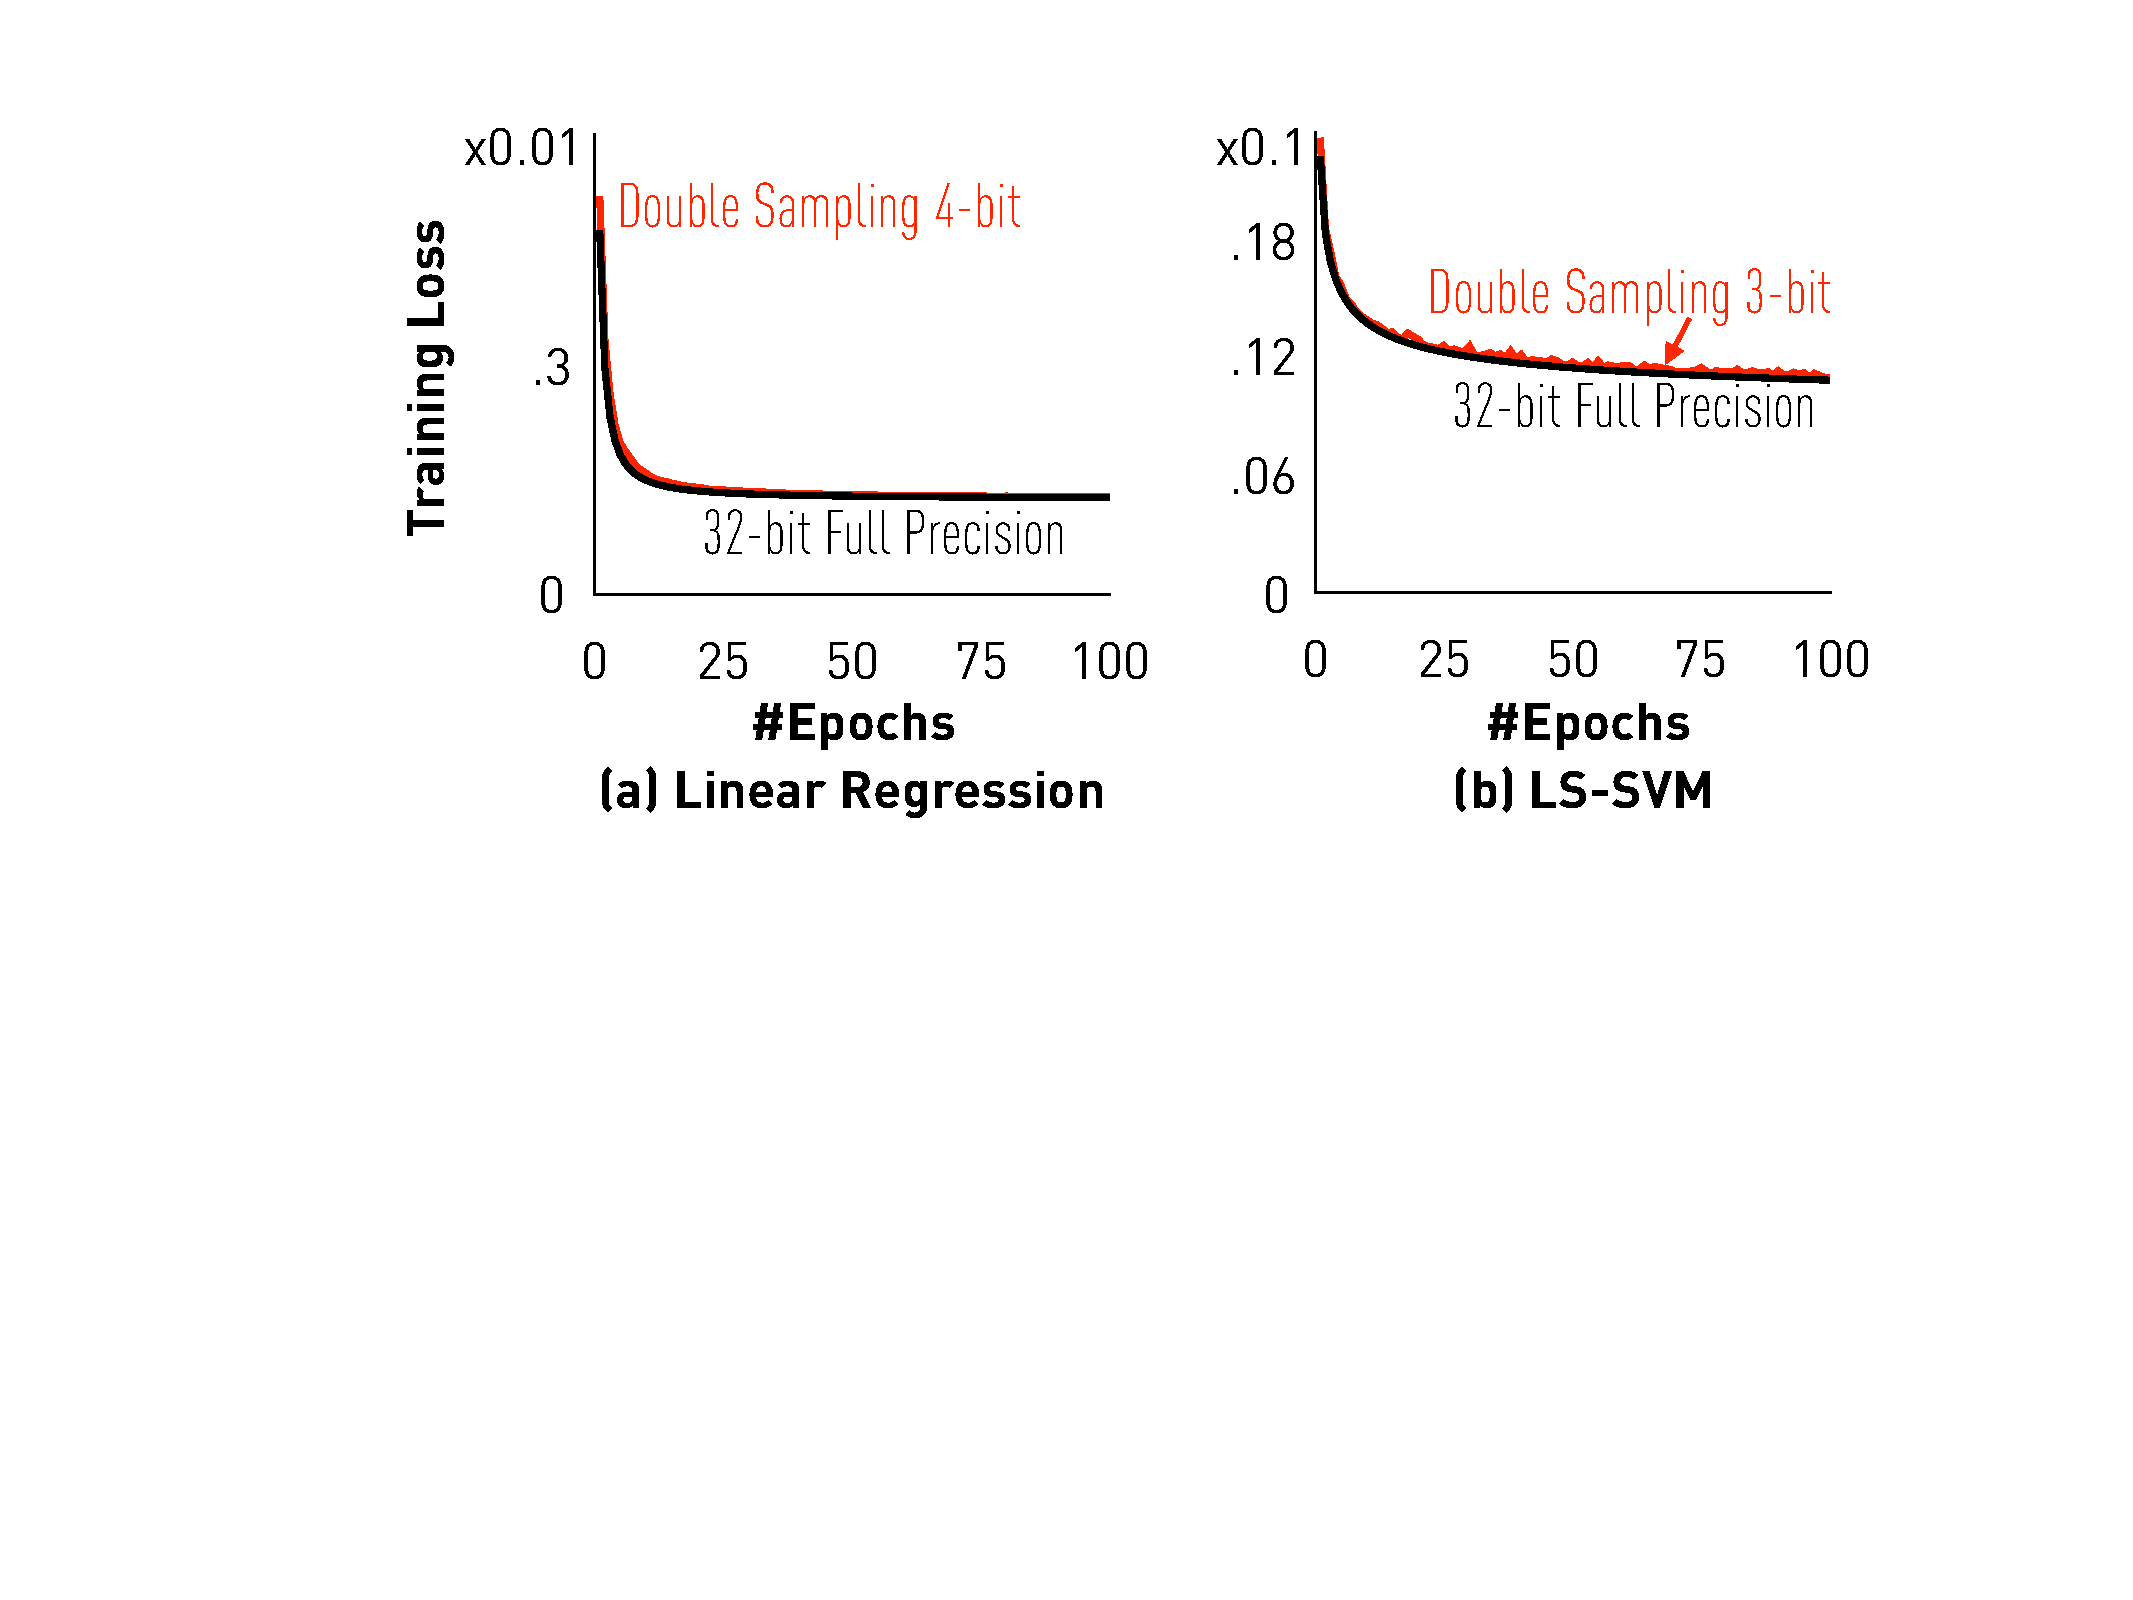
\includegraphics[width=\columnwidth]{final-experiments/linearmodel} 
\caption{Linear models with end-to-end low precision.}
\label{fig:convergence}
\end{figure}

\paragraph{Speedup}
We implemented our low-preicision framework for training a linear model on FPGA. We compare the time to converge to the same training loss with 32-bit FPGA implementation and the current fastest multi-thread CPU implementation, Hogwild!.

Figure~\ref{fig:speedup} shows that with our quantization framework
implementation on FPGA with quantized data, 
we get 6x-7x speed up compared to state-of-art
10-thread CPU or FPGA with full 32-bit floating point data. The speed of FPGA is bounded by memory-bandwidth, and by using our framework to quantize data, we save 8x memory-bandwith, which leads to 6x-7x speed up.
\begin{figure}[t]
\centering
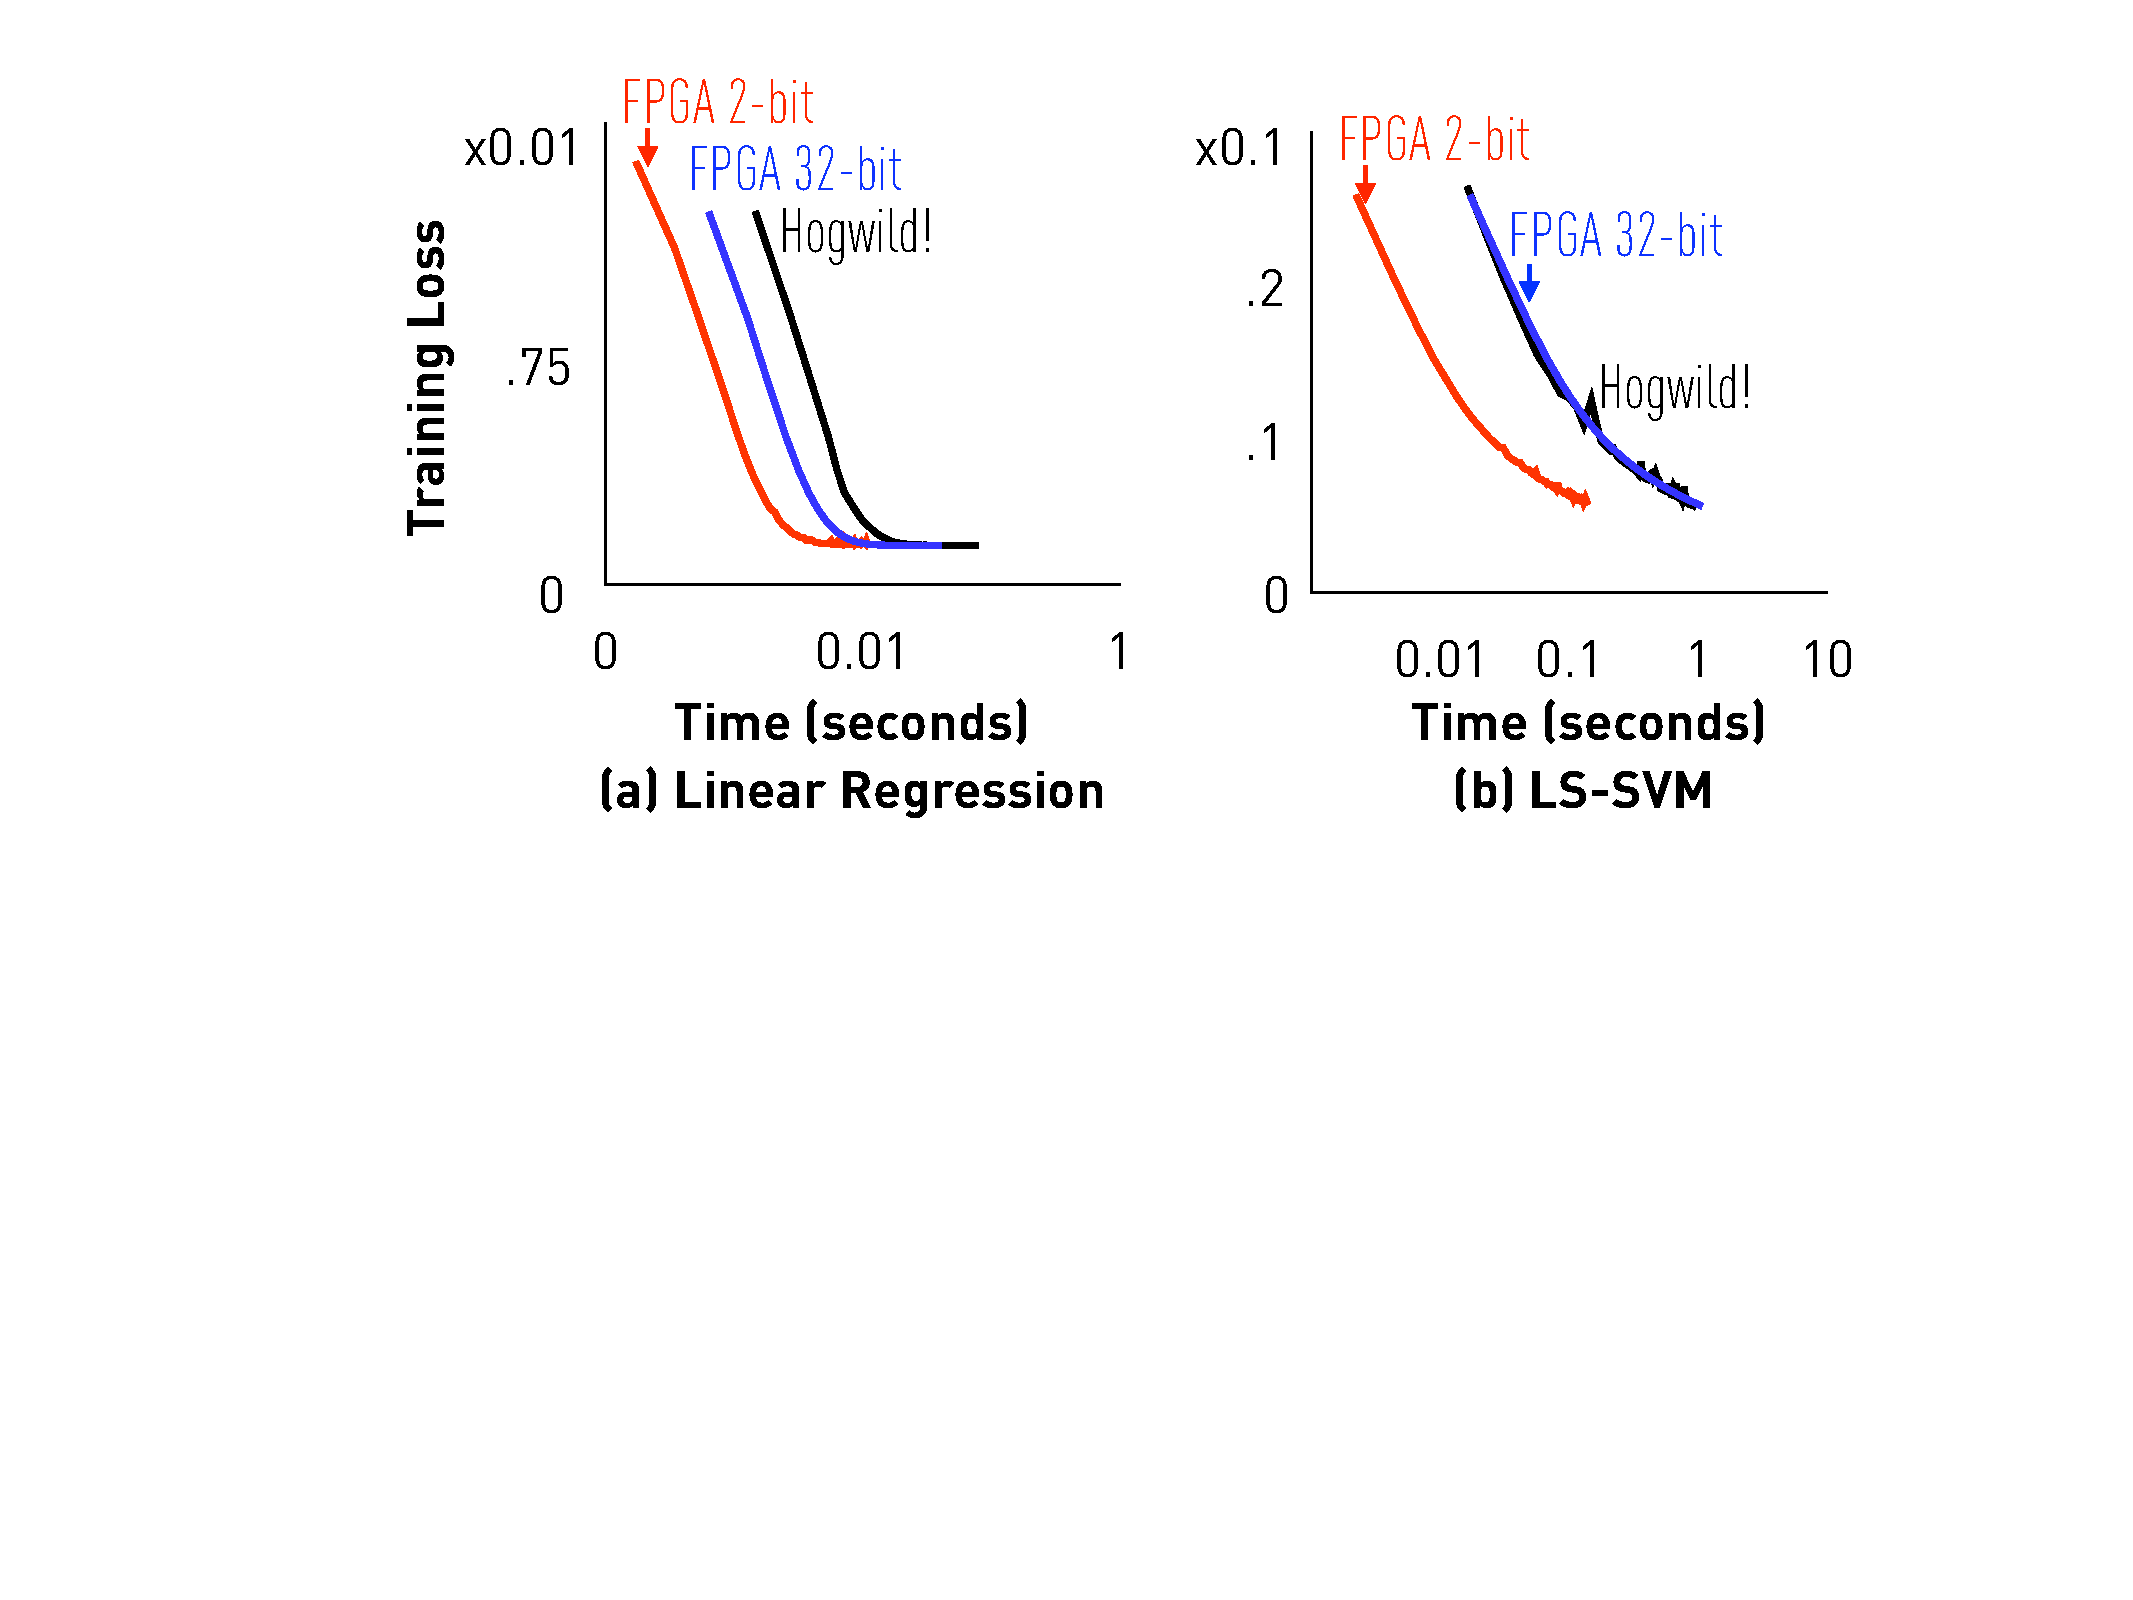
\includegraphics[width=\columnwidth]{final-experiments/linear-fpga} 
\caption{FPGA implementation of linear models.}
\label{fig:speedup}
\end{figure}

\subsection{Non-Linear Models}
In this section, we validate that: (1) ZipML 
converges to almost the same solution with comparable
empirical convergence rate for (i) SVM;
and (ii) Logistic Regression;
(2) If we use 8-bit deterministic rounding or naive stochastic rounding, we would also converge to the same solution for (i) SVM;
and (ii) Logistic Regression.

\paragraph{Chebyshev Approximations}
We run SGD to train models for SVM and logistic regression using:
(1) original 32-bit data and original gradient; (2) original 32-bit data and gradient approxiamted by Chebyshev polynomials;
(3) quantized data and gradient approxiamted by Chebyshev polynomails.
We compare the training loss and test accuracy in these 3 settings.

Figure~\ref{fig:chebyshev} shows that with Chebyshev polynomial approximation to sigmoid 
or sign function, our quantization framework
converges to close training loss with comparable
empirical convergence rate for both SVM and logistic regression
with only 3 to 5-bit data quantization. We also get no loss in test accuracy.

\begin{figure}[t]
\centering
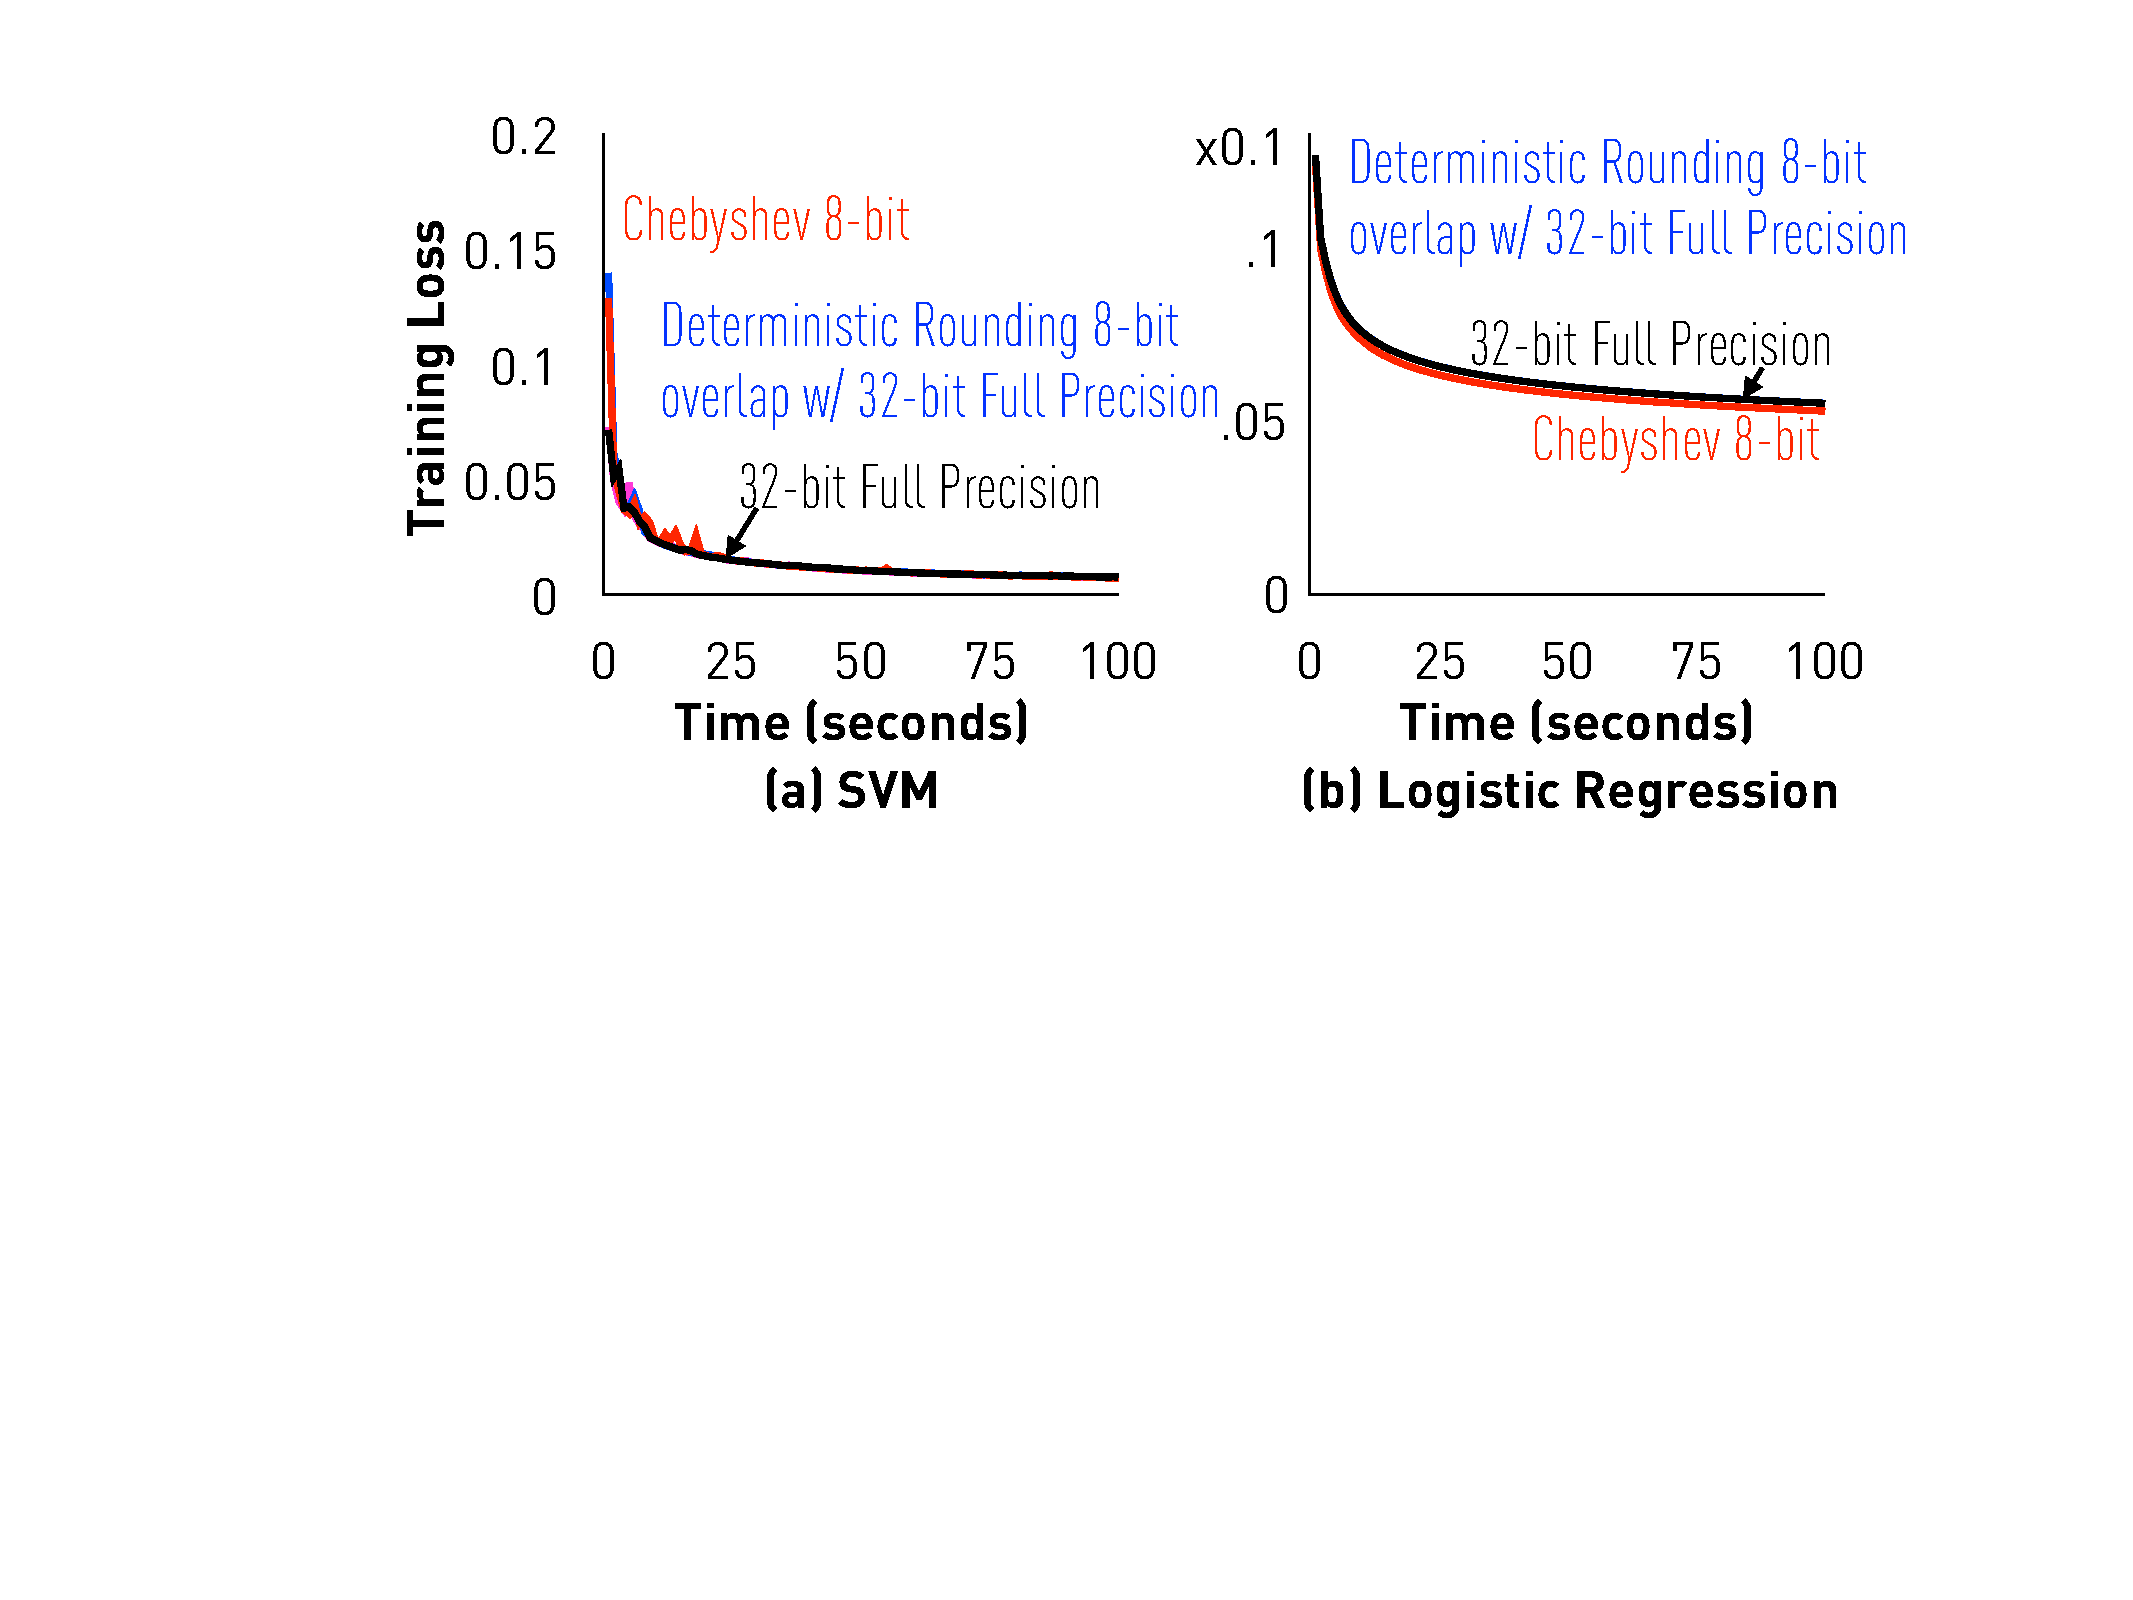
\includegraphics[width=\columnwidth]{final-experiments/chebyshev} 
\caption{Non-linear models with Chebyshev approximation.}
\label{fig:chebyshev}
\end{figure}

\paragraph{Negative Results}
We compare our previous result with naive 8-bit deterministic or stochastic rounding for data.

Figure~\ref{fig:vsnaive} shows that with 8-bit deterministic rounding or naive
stochastic rounding, SGD would also converge to same training loss with comparable
empirical convergence rate. However, we need to send multiple samples if we use the Chebyshev polynomial approximation. 
Even though these additional samples can be encoded efficiently (since they can only take a limited set of values), 
in practice the memory-bandwith savings of our framework
compared to simple 8-bit deterministic rounding are minor. 

\begin{figure}[t]
\centering
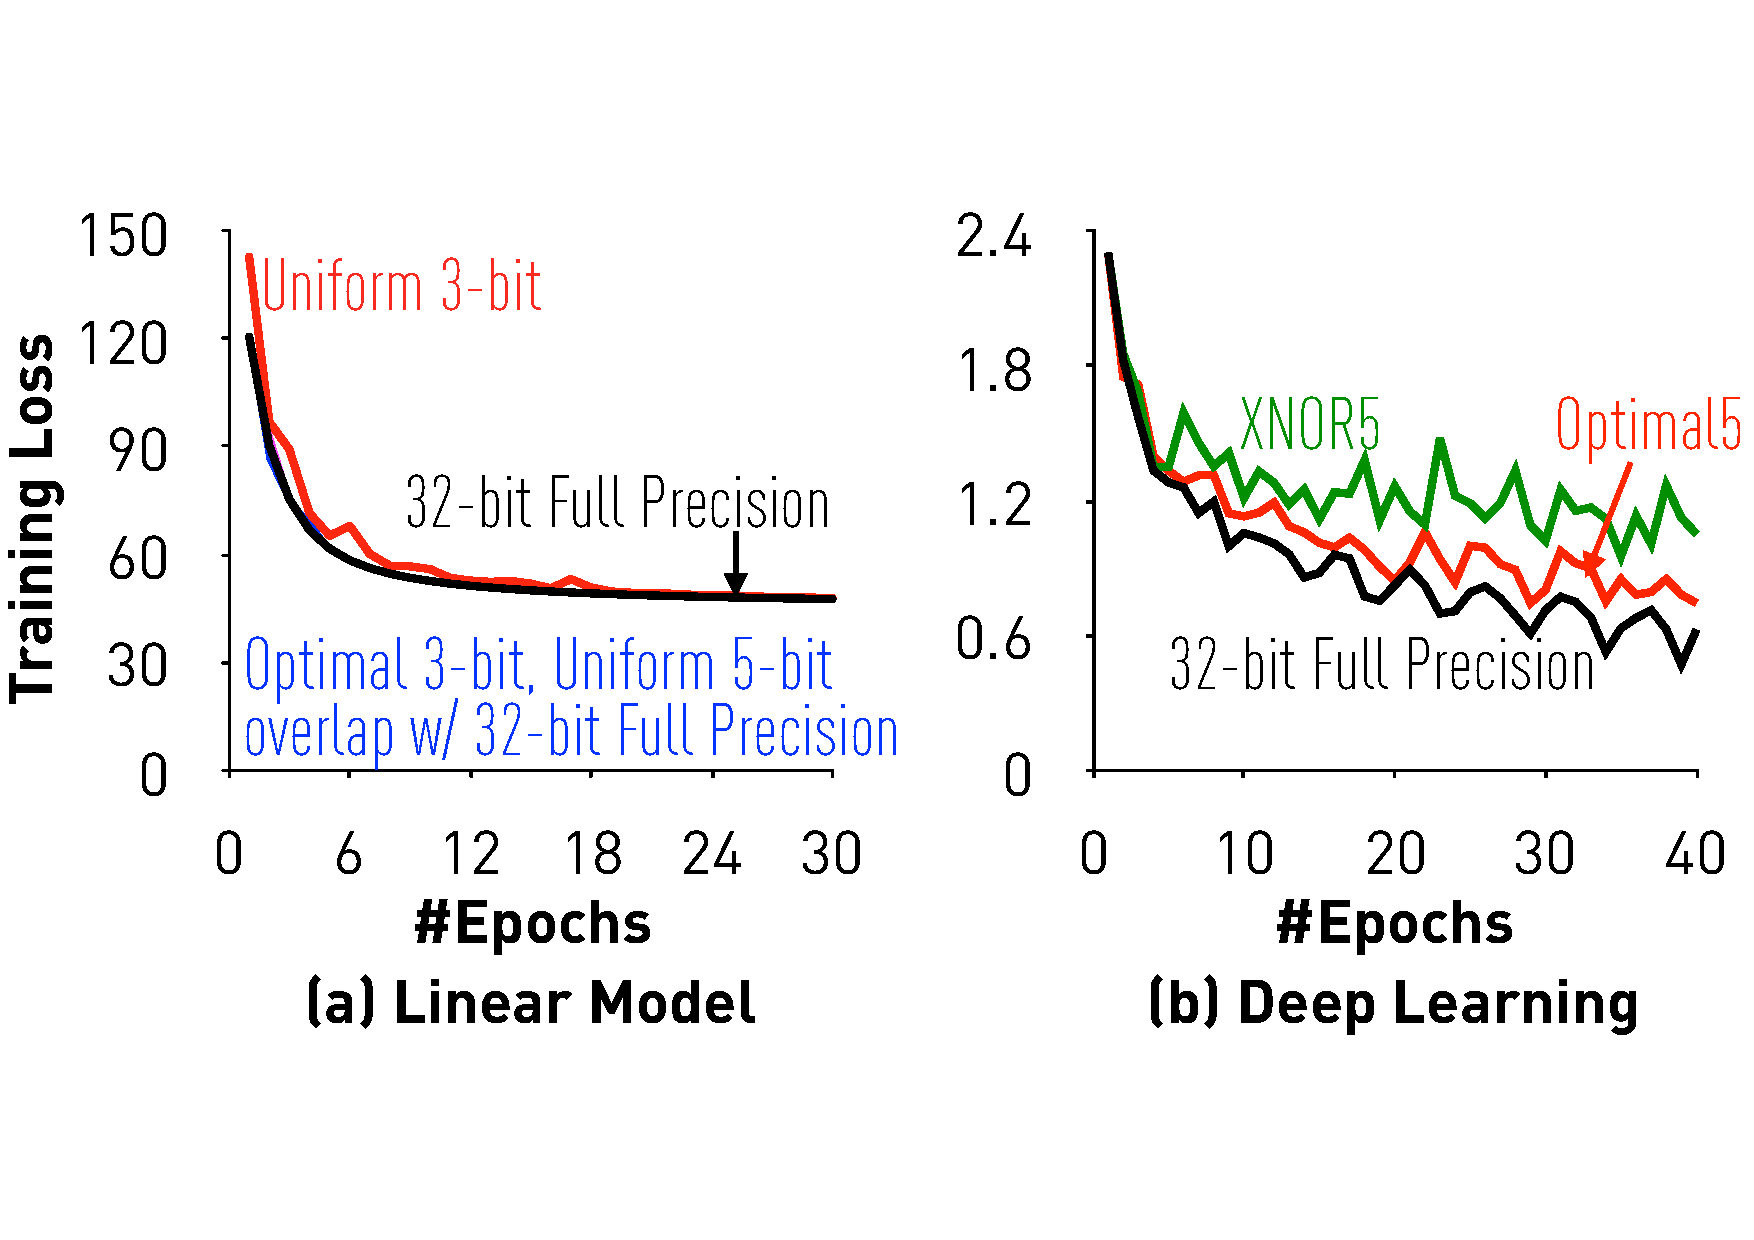
\includegraphics[width=\columnwidth]{final-experiments/optimal} 
\caption{Optimal quantization strategy.}
\label{fig:optimal}
\end{figure}

\subsection{Data-Optimal Quantization Strategy}
We validate that: with our data-optimal quantization strategy, 
SGD can converge to the same solution with comparable convergence rate with less bits 
compared to using uniform quantization levels. We compare the training loss of using data-optimal levels with 3-bit quantization and uniform levels with 3-bit and 5-bit quantization


Figure~\ref{fig:optimal}(a) shows that with our data-optimal quantization strategy, on this data set, it is enough to use 3-bit quantization. If we use the uniform quantization levels, we need at least 5-bit data quantization to get the same performance. We save almost half of the bits we need by just allocating markers wisely.


\subsection{Extensions to Deep Learning}

We validate that our data-optimal quantization
strategy can be used in training deep neural
networks. We take Caffe's CIFAR-10 tutorial
and compare four different quantization
strategies: (1) Full Precision, (2) BNN5, 
a BNN implementation that quantize data into
five uniformly chosen levels, and (3)
Optimal5, our quantization strategy with
five optimal quantization levels. As
shown in Figure~\ref{fig:optimal}(b), Optimal5
converges to a significantly lower training 
loss compared with BNN5. In terms of
testing accuracy, Optimal5 achieves a
near 10 points improvement over BNN5.
This illustrates the improvement
one can get by training neural network with
a carefully chosen quantization strategy.






\section{Related Work} 

There has been intensive study about ``low precision SGD''~\cite{DeSa:NIPS:2015,Alistarh:2016:ArXiv}. 
Most of them provide
theoretical guarantee when the gradients are quantized.
The model and input samples, on the other hand, are much more difficult
to analyze because of the non-linearity. In this paper, 
we
focus on the {\em end-to-end}
quantization for all components.

\vspace{-1em}
\paragraph{Low-Precision Deep learning.}

Low-precision training of deep neural networks has been studied
intensively and many heuristics work well for a subset of networks.
For example, OneBit SGD~\cite{Frank:2014:Interspeech} provides
a gradient compression heuristic developed in the context of deep 
neural networks for speech recognition. There are successful 
application of end-to-end quantization to training neural networks
resulting in little to no quality loss~\cite{hubara2016quantized,
rastegari2016xnor,zhou2016dorefa,miyashita2016convolutional,li2016ternary,gupta2015deep}. These work quantize weights, activations, and gradients 
to low-precision (e.g., 1-bit) and revise the backpropagation 
algorithm to be aware of the quantization function.
The empirical success of these work inspired this paper, in which we try
to provide a {\em theoretical} understanding of end-to-end low-precision
training for machine learning models.
Another line of research concerns about inference and model
compression of a pre-trained model~\cite{vanhoucke2011improving,gong2014compressing,Han:2016:ICLR,lin2016fixed,kim2016bitwise,kim2015compression,wu2016quantized}.
In this paper, we focus on training and leave the study of
inference as future work.

\vspace{-1em}
\paragraph{Low-Precision Linear Models.}

Quantization is a fundamental topic studied by the
DSP community, and there have been research related to
linear regression models in the presence of quantization
error or other type of noises. For example,
\citet{Gopi:2013:ICML} studied compressive sensing
with quantized measurement, and the \textcolor{red}{XXXXX}
algorithm focuses on getting a high-precision solution
with low-precision computation. Also, the
classic errors-in-variable model~\cite{Hall:2008:Book}
could also be related if quantization is treated 
as a source of ``error''. In this paper, we scope
ourselves in the context of stochastic gradient descent, 
and our insights go beyond simple linear models.

\vspace{-1em}
\paragraph{Other Related Work.} Precision of data
representation is a key design decision to make
for configurable hardwares such as FPGA. There have
been attempts to
lower the precision when training machine learning models
on these hardware~\cite{Kim:2011:ICASSP}. 
These results are mostly empirical; We
aim at providing a theoretical understanding, which 
enables new practical algorithms that are not covered 
by these work.



\cleardoublepage

\bibliographystyle{icml2017}
\bibliography{low-precision.bib}




%\begin{proof}
%We have that 
%\[
%\E_{Q_1, Q_2}(\|\g_k\|^2) = \E_{Q_1, Q_2} [\| Q_1 (\a_k, s) (Q_2 (\a_k, s)^\top \x + b_k) \|_2^2].
%\]
%Next we have
%\begin{align*}
%    \E_{Q_1, Q_2} [\| Q_1 (\a_k, s) (Q_2 (\a_k, s)^\top \x + b_k) \|_2^2] &= \E_{Q_2} \left[ \E_{Q_1} [ (Q_2 (\a_k, s)^\top \x + b_k)^2 Q_1 (\a_k, s)^\top Q_1 (\a_k, s)] \right] \\
%    &= \E_{Q_1}[ \| Q_1( \vec{a}_k, s) \|_2^2 ] \cdot \E_{Q_2} [\| \a_k (Q_2 (\a_k, s)^\top \x + b_k)\|_2^2 ] \\
%    &\leq^{\mathrm{Lemma}~\ref{lem:quant-facts}} r M_a^2 \cdot \E [(Q_2 (\a_k, s)^\top \x + b_k)^2 ] \\
%    &= r M_a^2 \left( \E [(Q_2 (\a_k, s)^\top \x)^2] + 2 b_k \E [Q_2 (\a_k, s)^\top \x] + b_k^2 \right) \\
%    &= r M_a^2 \left( \E [(Q_2 (\a_k, s)^\top \x)^2] + 2 b_k \a_k^\top \x + b_k^2 \right)
%\end{align*}
%Moreover, we have
%\begin{align*}
%    E [(Q_2 (\a_k, s)^\top \x)^2] &= \x^\top \left( \E \left[ Q_2 (\a_k, s) Q_2 (\a_k, s)^\top \right] \right) \x \\
%    &= \x^\top (\a_k \a_k^\top + D) \x^\top \\
%    &\leq (\a_k^\top \x)^2 + \| D \|_{\mathrm{op}} \| \x \|_2^2 \; ,
%\end{align*}
%where $D = \mathrm{diag}_i [ (\E[Q_2 (\a_k, s)_i^2]) - (\a_k)_i^2 ] =\mathrm{diag}_i [ \mathrm{Var} [Q_2 (\a_k, s)_i] ].$ Further, we have that $\| D \|_{\mathrm{op}}  \leq M_a^2 / s^2$.
%Therefore we have that:
%\begin{align*}
%     \E_{Q_1, Q_2} [\| Q_1 (\a_k, s) (Q_2 (\a_k, s)^\top \x + b_k) \|_2^2]  &\leq r M_a^2 \left( (\a_k^\top \x)^2 + \frac{M_a^2}{s^2} R^2 + 2 b_k \a_k^\top \x + b_k^2  \right) \\
%    &= r \left( \| \g'_k \|_2^2 \cdot \frac{M_a^2}{\| \a_k \|_2^2} + \frac{A^2 M_a^2 R^2}{s^2} \right) \,
%\end{align*}
%as claimed, since $\| \g'_k \|_2^2 = \| \a_k \|_2^2 (\a_k^T \x + b_k)^2$.
%\end{proof}

%\begin{proof}
%    Observe that $\| \g_k - \nabla f(\x_k) \|_2^2 = \| \g_k - \g'_k \|_2^2 + 2 (\g_k - \g'_k)^\top (\g'_k - \nabla f(\x_k)) + \| g'_k + \nabla f(\x_k) \|_2^2$.
%    Since $\E [(\g_k - \g'_k)^\top (\g'_k - \nabla f(\x_k))] = 0$, and by assumption $\E [ \| g'_k + \nabla f(\x_k) \|_2^2] \leq \sigma^2$, it suffices the bound the expectation of the first term.
%    We have
%    \[
%     \E \left[ \| \g_k - \nabla f(\x_k) \|_2^2 \right] \leq 2 \sigma^2 + 2\E_{\g'_k} \left[ \E_{Q_1, Q_2} [ \| \g'_k - \g_k \|_2^2 \left| \right. \g'_k ] \right] \; .
%    \]
%    Since $\E_{Q_1, Q_2} [\g_k | \g'_k] = \g'_k $, we have that 
%    \begin{align*}
%    \E_{Q_1, Q_2} [ \| \g'_k - \g_k \|_2^2 \left| \right. \g'_k ] &= \E_{Q_1, Q_2} [\| \g_k \|_2^2 | \g'_k] - \| \g'_k \|_2^2 \\
%    &\leq \left(r \frac{M_a^2}{\| \a_k \|_2^2} - 1\right) \| \g'_k \|_2^2 + \frac{r A^2 M_a^2 R^2}{s^2} \; ,
%    \end{align*}
%    from which the corollary follows.
%\end{proof}

%\begin{proof}
%We have
%\begin{align*}
%    \E [\| \g_k \|_2^2] &= \| \a_k \|_2^2 \E \left[\left( \a_k^\top Q( \x, s)  + b_k \right)^2 \right] \\
%    &= \| \a_k \|_2^2 \left( a_k^\top \E[Q(\x, s) Q(\x, s)^\top] a_k + 2 b_k \E[Q(\x, s)^\top \a_k] + b_k^2 \right) \\
%    &= \| \a_k \|_2^2 \left( a_k^\top \E[Q(\x, s) Q(\x, s)^\top] a_k + 2 b_k \x^\top \a_k + b_k^2 \right) \; .
%\end{align*}
%As we had previously for double sampling, we have
%\begin{align*}
%    \a_k^\top \left( \E \left[ Q_2 (\x, s) Q_2 (\x, s)^\top \right] \right) \a_k &= \a_k^\top (\x \x^\top + D) \a_k^\top \\
%    &\leq (\a_k^\top \x)^2 + \| D \|_{\mathrm{op}} \| \a_k \|_2^2 \; ,
%\end{align*}
%where as before we have that $D$ consists of diagonal elements $\E[Q_2 (\x, s)_i^2]) - (\x)_i^2 = [\mathrm{Var} [Q_2 (\x, s)_i]] \leq M_x^2 / s^2$.
%Hence altogether we have
%\[
%\E [\| \g_k \|_2^2] \leq \| \g'_k \|_2^2 + \frac{A^4 M_x^2}{s^2} \; ,
%\]
%as claimed.
%\end{proof}













\iffalse

%\begin{figure}[t]
%\centering   
%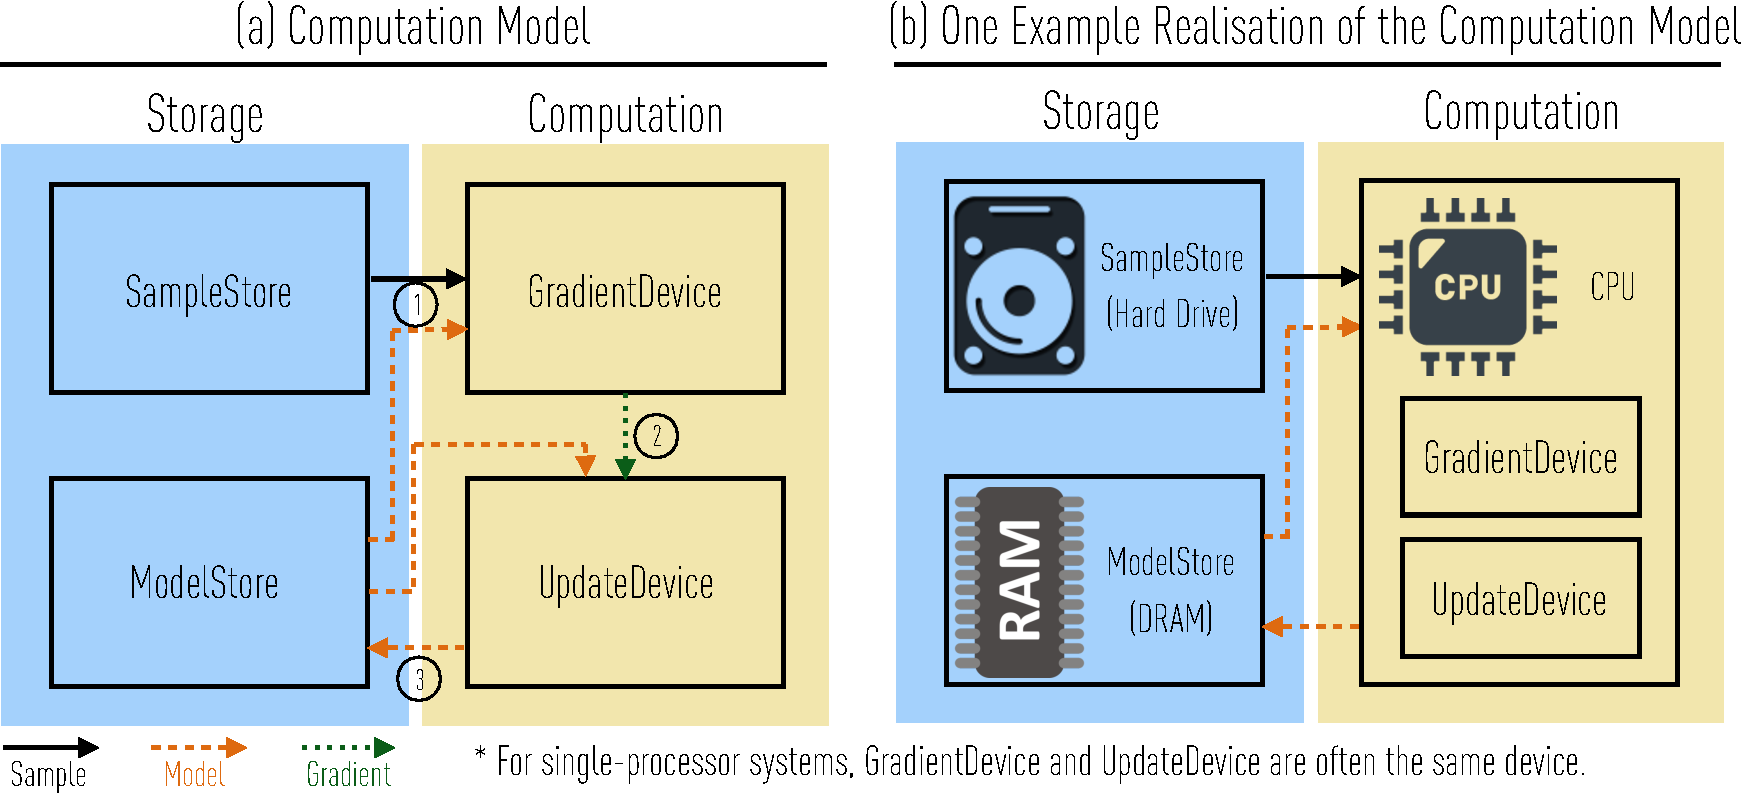
\includegraphics[width=0.5\textwidth]{compmodel-pdfcrop}
%\caption{A Schematic Representation of the Computation Model and (b) An Example %Realisation
%of the Computation Model. Three types of
%data, namely (1) sample, (2) model, and (3)
%gradient, moves in the system in three
%steps as illustrated in (a). Given
%different parameters of the computation model,
%such as computational power and memory bandwidth, the system bottleneck may
%vary. For example, in 
%realisation (b) having a hard drive, DRAM, and a
%modern CPU, it is likely that the  bottleneck when training 
%a dense generalized linear model is the
%memory bandwidth between SampleStore
%and GradientDevice.}
%\label{fig:model}
%\end{figure}


%\begin{figure}[h]
%\centering
%   
%    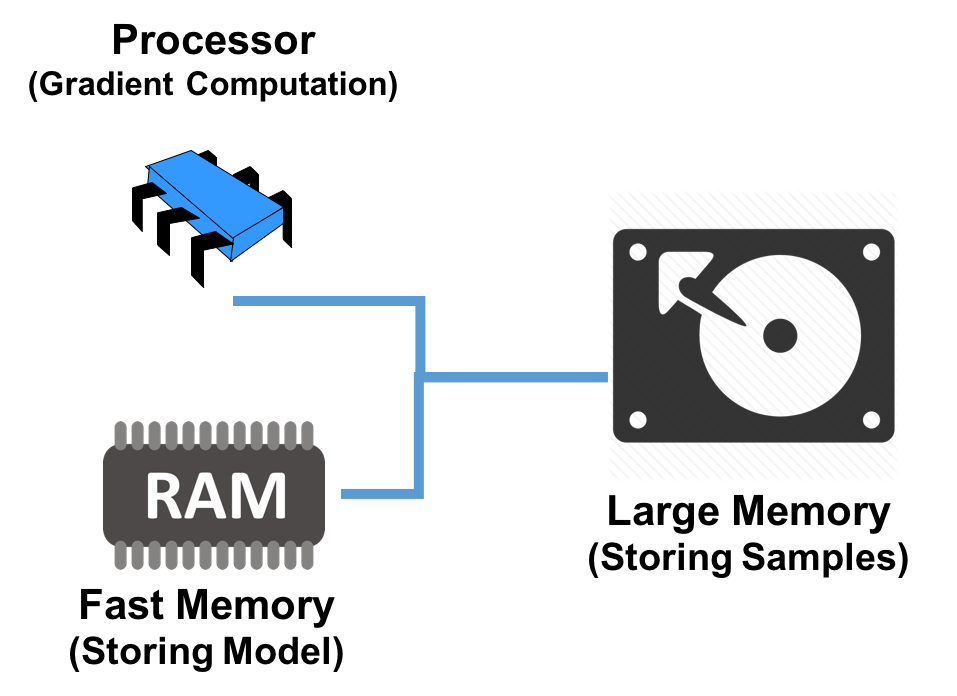
\includegraphics[scale=0.4]{schematic}
%    
%\caption{Simple Schematic of the %Computational Model}
%\label{fig:model}
%\end{figure}

\section{Guarantees for SGD}
In this paper we consider SGD, a general family of stochastic first order methods for finding the minima of convex (and non-convex) functions.
Due to its generality and usefulness, there is a vast literature on SGD in a variety of settings, with different guarantees in all of these settings.
Our techniques apply fairly generally in a black box fashion to many of these settings, and so for simplicity we will restrict our attention to a fairly basic setting.
For a more comprehensive treatment, see \cite{Bubeck15}.

Throughout the paper, we will assume the following setting in our theoretical analysis.
Let $\mathcal{X} \subseteq \R^n$ be a known convex set, and let $f: \mathcal{X} \to \R$ be differentiable, convex, and unknown.
We will assume the following, standard smoothness condition on $f$:
\begin{definition}[Smoothness]
Let $f: \R^n \to \R$ be differentiable and convex.
We say that it is $L$-smooth if for all $\x, \y \in \R^n$, we have
\[0 \leq f(\x) - f(\y) - \nabla f(\y)^T (\x - \y) \leq \frac{L}{2} \| \x - \y \|_2^2 \; .\]
\end{definition}

We assume repeated access to stochastic gradients, which on (possibly random) input $\vec{x}$, outputs a direction which is in expectation the correct direction to move in.
Formally:
\begin{definition}
Fix $f: \mathcal{X} \to \R$.
A \emph{stochastic gradient} for $f$ is a random function $g (\x)$ so that $\E [g (\x) ] = \nabla f( \x)$.
%A \emph{stochastic oracle} for $f$ is an oracle which on (possibly random) input $\vec{x}$, outputs a stochastic gradient for $f$ at $\vec{x}$.
We say the stochastic gradient has second moment at most $B$ if $\E [\| g \|_2^2] \leq B$ for all $\x \in \mathcal{X}$.
We say it has variance at most $\sigma^2$ if $\E [\| g (\x) - \nabla f(\x) \|_2^2] \leq \sigma^2$ for all $\x \in \mathcal{X}$. 
\end{definition}

Under these conditions, the following convergence rate for SGD is well-known:

\begin{theorem}[e.g. \cite{Bubeck15}, Theorem 6.3]
Let $\mathcal{X} \subseteq \R^n$ be convex, and let $f: \mathcal{X} \to \R$ be an unknown, convex, and $L$-smooth.
Let $\x_0 \in \mathcal{X}$ be given, and let $R^2 = \sup_{\x \in \mathcal{X}} \| \x - \x_0 \|^2$.
Suppose we run projected SGD on $f$ with access to independent stochastic gradients with variance bound $\sigma^2$ for $T$ steps, with step size $\eta_t = 1 / ( L + \gamma^{-1})$, where $\gamma = \frac{R}{\sigma} \sqrt{\frac{2}{T}}$, and
\begin{equation}
\label{eq:sgd-conv}
T = O \left( R^2 \cdot \max \left( \frac{2 \sigma^2}{\epsilon^2} , \frac{L}{\epsilon} \right) \right) \; .
\end{equation}
Then $\E \left[ f \left( \frac{1}{T} \sum_{t = 0}^T \x_t \right) \right] - \min_{\x \in \mathcal{X}} f(\x) \leq \epsilon$.
\end{theorem} 

In particular, note that the complexity the SGD method is mainly controlled by the variance bound $\sigma^2$ we may obtain. If $\sigma = 0$, the complexity is consistent with the stochastic gradient.


\subsection{Randomized Quantization}

In this section, we give a procedure to quantize a vector or real values randomly, reducing its information content. We will denote this quantization function by $Q(\vec{v},s)$, where $s\geq 1$ is the tuning parameter. 
Let $M(\vec{v}): \R^n \rightarrow \R^n$ be a positive scaling function such that, for $\vec{v}\in \R^n$, $\frac{\vec{v}_i}{M_i(\vec{v})} \in [-1, 1]$, where $M_i(\vec{v})$ denotes the $i$th element of $M(\vec{v})$.
For $\vec{v} \neq \vec{0}$ we define

\begin{equation}
Q_i(\vec{v},s) = M_i(\vec{v}) \cdot \sgn{\vec{v}_i} \cdot \mu_i(\vec{v},s) \; , \label{equ:quant2}
\end{equation}
where $\mu_i(\vec{v},s)$'s are independent random variables defined as follows. 
Let $0 \leq \ell < s$ be an integer such that $|\vec{v}_i|/M_i(\vec{v}) \in [ \ell / s, (\ell + 1) / s ]$, that is, $\ell = \lfloor s |\vec{v}_i|/\| \vec{v} \| \rfloor$. 
Here, $p(x,s) = x s - \ell$ for any $x \in [0,1]$.
Then 
\[
\mu_i(\vec{v},s) = \left\{ \begin{array}{ll}
         \ell / s & \mbox{with probability $1 - p\left(\frac{|\vec{v}_i|}{M(\vec{v})},s\right)$};\\
         (\ell + 1) / s & \mbox{otherwise}. \end{array} \right.
\]
If $\vec{v} = \vec{0}$, then we define $Q(\vec{v},s) = \vec{0}$.
For any such choice of $M_i$, we have the following properties, which generalize Lemma 3.4 in~\cite{QSGD}.
The proofs follow immediately from those in \cite{QSGD}, and so we omit them for conciseness.
\begin{lemma}
\label{lem:quant-facts}
 For any $\vec{v} \in \R^n$, we have that 
 \begin{itemize} 
 \item (Sparsity) $\E[ \|Q(\vec{v}, s)\|_0]\leq
 s^2 +\sqrt{n}$ , 
 \item (Unbiasedness) $\E [Q (\vec{v},s)] = \vec{v}$ , and
 \item (Second Moment Bound) 
$\E [\| Q (\vec{v},s) \|_2^2] \leq r M^2$, where $M = \max_i M_i (\vec{v})$, and 
\[
r = r(s) = \left( 1 + \frac{1}{s^2} \sum_{i = 1}^n p\left( \frac{|\vec{v}_i|}{M_i },s \right) \right) \; .
\]
 \end{itemize}
\end{lemma}


We now discuss different choices of the scaling function $M_i(\vec{v})$.

\paragraph*{``Row Scaling''}

One obvious choice that was suggested in \cite{QSGD} is to have $M_i(\vec{v}) = \| \vec{v} \|_2$, in this way, we
always have $\frac{\vec{v}_i}{M_i(\vec{v})} \in [-1, 1]$ and all $M_i(\vec{v})$ are the same
such that we can store them only once.
When the 
In the following, we will often use the version with $s = 1$, which is as follows. 
\begin{equation}
\label{equ:quant1}
Q_i(\vec{v}) = \| \vec{v} \|_2 \cdot \sgn{\vec{v}_i} \cdot \mu_i (\vec{v}) \; ,
\end{equation}
where $\mu_i(\vec{v})$'s are independent random variables such that $\mu_i(\vec{v}) = 1$ with probability $|\vec{v}_i| / \| \vec{v} \|_2$, and $\mu_i(\vec{v}) = 0$, otherwise. If $\vec{v} = \vec{0}$, we define $Q(\vec{v}) = \vec{0}$. 
%
Obviously, if
all vectors $\vec{v}$ are scaled to have unit $\ell_2$ norms, $M(\vec{v}) \equiv 1$
and therefore, we can also omit this term.
Moreover, it was shown in \cite{QSGD} that for this choice of $M_i$, the function $r$ can be upper bounded by
\[
r(s) \leq \rrow (s) = 1 + \min\left( \frac{n}{s^2}, \frac{\sqrt{n}}{s} \right) \; .
\]

\paragraph*{``Column Scaling''}
Let $\vec{v} \in \R^n$ be a sample and $V \subset \R^n$ be the set of sample vectors. 
%Another choice, especially when $\vec{v} \in \R^n$ is an input sample and 
We can obtain the upper and lower bound for each feature, that is,
%$the {\em constant} for each $\vec{v}_i$ such that Another choice, especially when $\vec{v} \in \R^n$ is an input sample and we know the {\em constant} for each $\vec{v}_i$ such that 
\[
\text{min}_i \le \vec{v}_i \le  \text{max}_i\quad \vec{v} \in V
\]
is to have $M_i(\vec{v}) = \max(|\text{min}_i|, |\text{max}_i|)$.
When the input samples are stored as a matrix in which each row corresponds
two a vector $\vec{v}$, getting $\min_i$ and $\max_i$
is just to getting
the $\min$ and $\max$ for each column (feature).
Using this scheme, all input samples can share the same
$M_i(\vec{v})$ and thus can be easily stored in cache when all
input samples are accessed sequentially (like in SGD).


\paragraph*{Choice between Row Scaling and Column Scaling}

In this working paper, we make the following choices regarding row scaling
and column scaling and leave the more general treatment to future work.
For all input samples, we always use column scaling because it is easy
to calculate $M_i$ which does not change during training. For all gradients
and models, we use row scaling because the range of values is more dynamic.


\section{Extension to Classification Models}


%\todo{Proof}

\section{Experiments} \label{sec:exp}

In this section, we validate that ZipML 
converges to the same solution with comparable
empirical convergence rate for a range of
statistical models: (1) linear regression;
(2) least squares support vector machines;
(3) support vector machines;
and (4) linear regression. We further validate that
with our data-optimal quantization strategy, we can use
less bits to get the same convergence speed
We validate this claim on a range of real-world
and synthetic data sets, and study the impact
of the number of bits at which we quantize for each task.

\subsection{Experimental Setup}

\paragraph{Datasets} 
We used a synthetic dataset with 10000 samples and 100 features for Linear Regression and we used gisette dataset~\cite{guyon2004result} with 6000(1000) training(testing) samples and 5000 features for classification problems(Least Sqaure SVM, SVM and Logistic Regression).

\paragraph{Metrics} To measure the quality of training,
we measured the training loss after each training epoch. For classification tasks, we also measured test accuracy.

\paragraph{Protocol} We run ZipML on each dataset, with the diminishing step_size, where the real step_size is ${initial\_step\_size/k}$, where k is the current number of epoch. 

\subsection{Linear Regression}
We first validate that ZipML 
converges to the same solution with comparable
empirical convergence rate for \emph{linear regression}.
We show the results for \texttt{cadata} in Figure~\ref{fig:lrcadata}, the results for \texttt{cpusmall} in Figure~\ref{fig:lrcpusmall}, the results for \texttt{music} in Figure~\ref{fig:lrmusic}, and the results for \texttt{synthetic} in Figure~\ref{fig:lr20easy} to \ref{fig:lr160hard}.

Figure~\ref{fig:lrcadata}-\ref{fig:lr160hard} show that for all datasets we choose and all stepsizes we run, our quantization framework
converges to the same solution with comparable
empirical convergence rate. 

Moreover, we can see that for a small number of features, Figure~\ref{fig:lrcadata}-\ref{fig:lrcpusmall}, each with 8 and 12 features, 3-bit quantization is good enough to get the same solution at a comparable rate, enabling a 10x reduction in the amount of data movement.

For datasets with more features, Figure~\ref{fig:lrmusic} and \ref{fig:lr160hard}, with 90 and 160 features respectively, we need at most 7 bits resolution (Figure~\ref{subfig:musicdgm}) to get the same solution. In most cases, a 5-bit quantization is enough for linear regression task, leading to a 6x reduction in data movement.

\begin{figure}[h]
\centering

    \begin{subfigure}[h]{.3\columnwidth}
    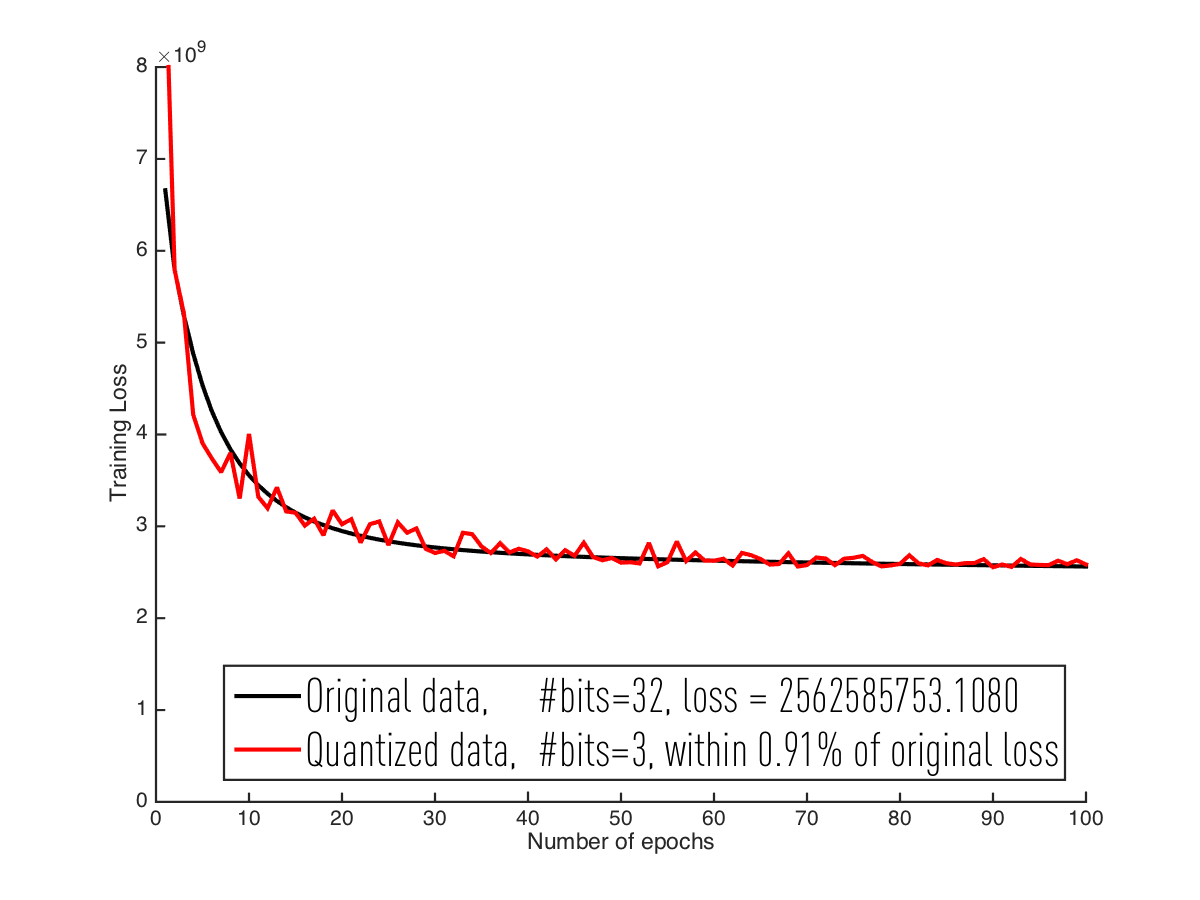
\includegraphics[width=\columnwidth]{lr/real/cadata/d01}
    \caption{Quantized data, initial stepsize = 0.1, 3-bit quantization}
    \end{subfigure}
    \begin{subfigure}[h]{.3\columnwidth}
    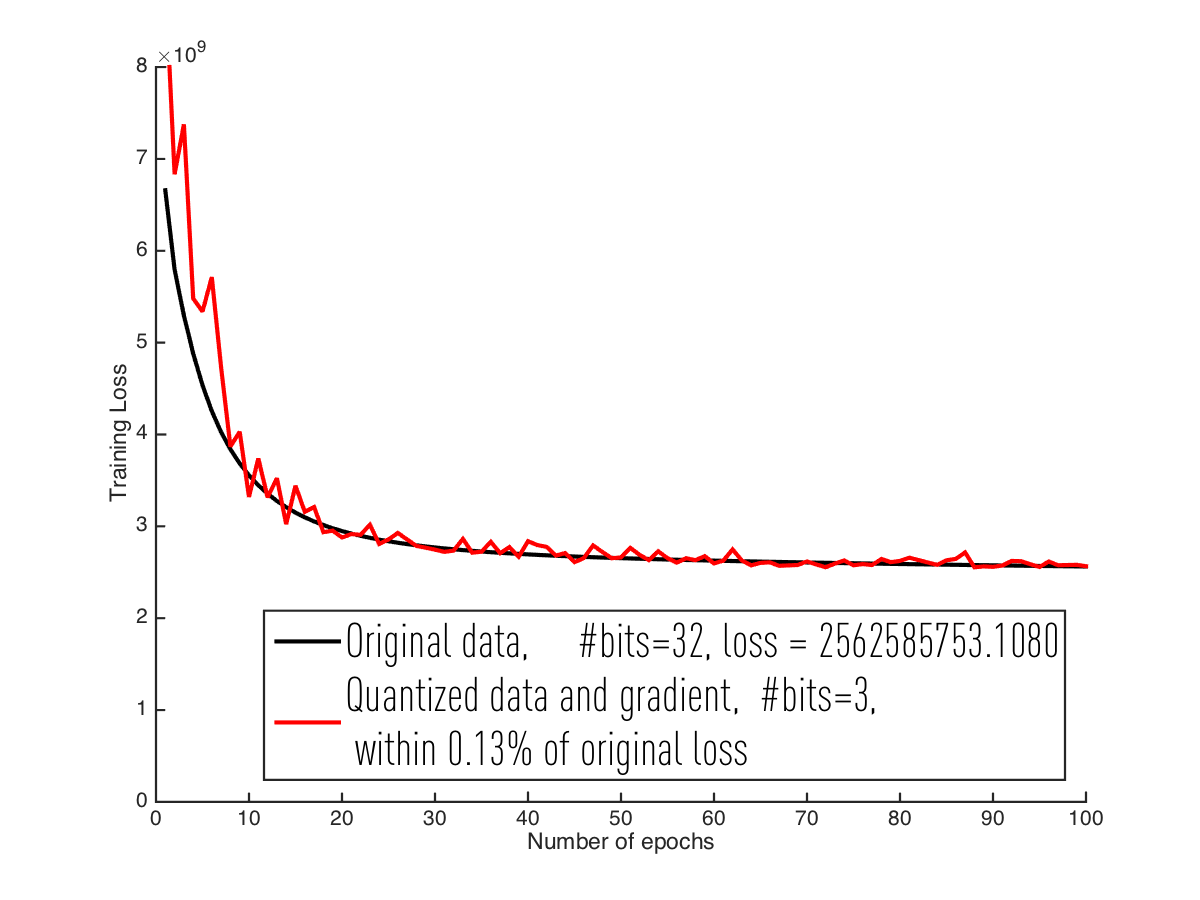
\includegraphics[width=\columnwidth]{lr/real/cadata/dg01}
    \caption{Quantized data and gradient, initial stepsize = 0.1, 3-bit quantization}
    \end{subfigure}
    \begin{subfigure}[h]{.3\columnwidth}
    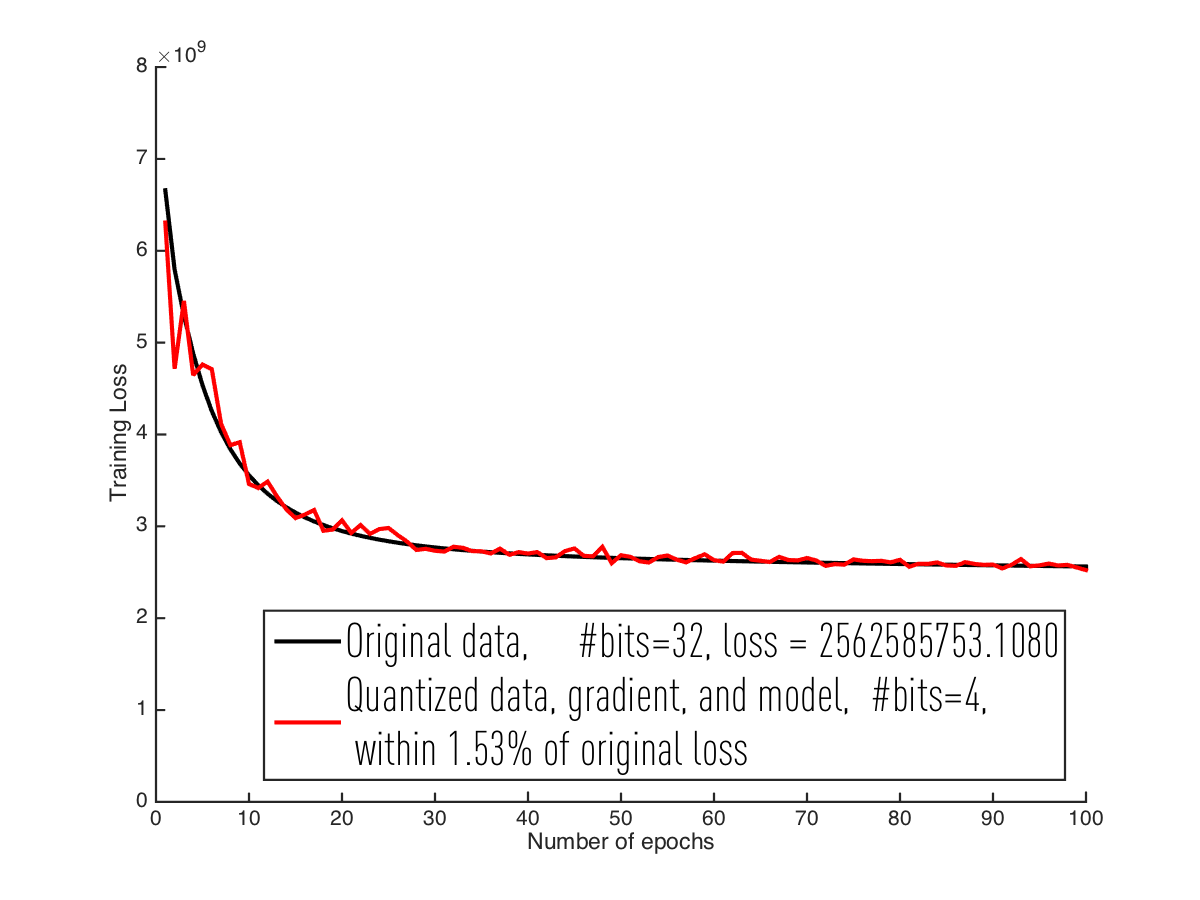
\includegraphics[width=\columnwidth]{lr/real/cadata/dgm01}
     \caption{Quantized data, gradient, and model, initial stepsize = 0.1, 4-bit quantization}
    \end{subfigure}
    
    \begin{subfigure}[h]{.3\columnwidth}
    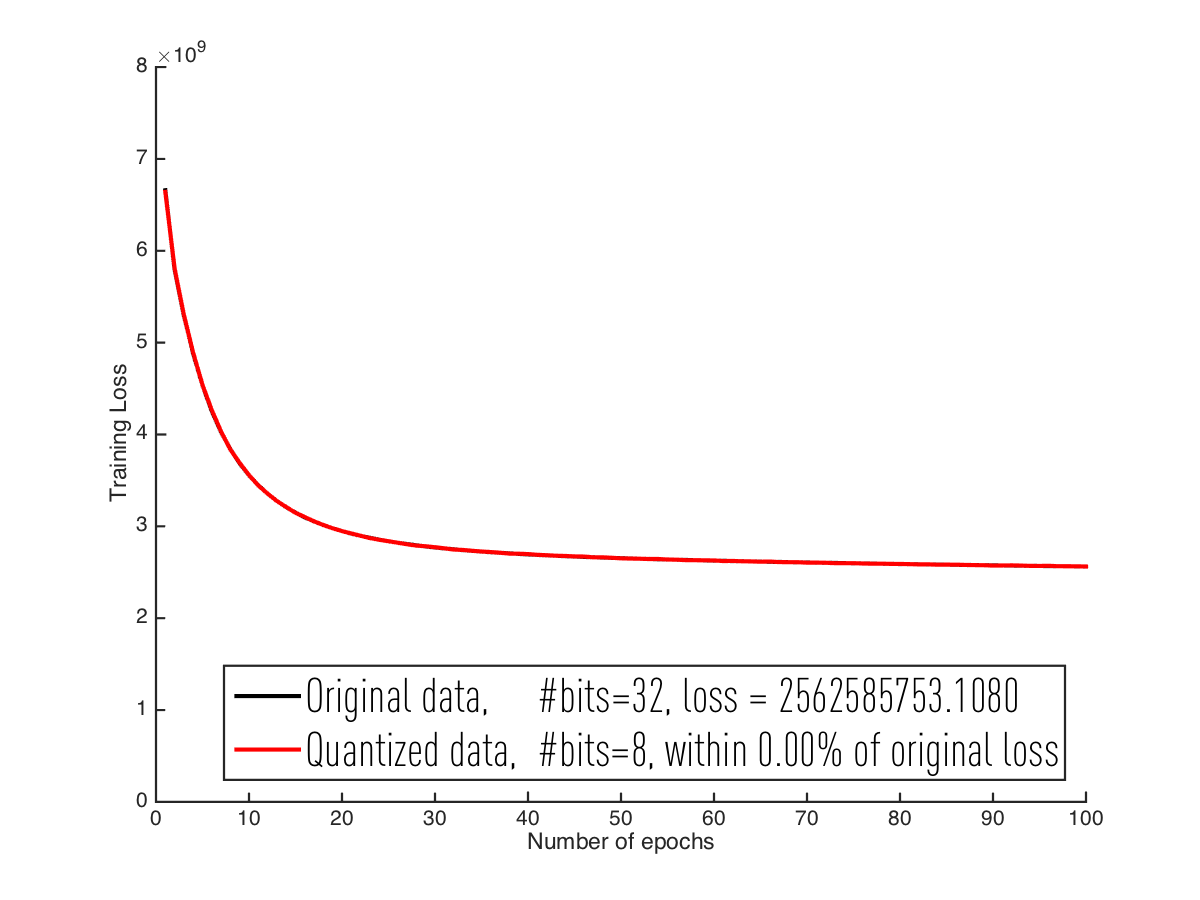
\includegraphics[width=\columnwidth]{lr/real/cadata/8d01}
    \caption{Quantized data, initial stepsize = 0.1, 8-bit quantization}
    \end{subfigure}
    \begin{subfigure}[h]{.3\columnwidth}
    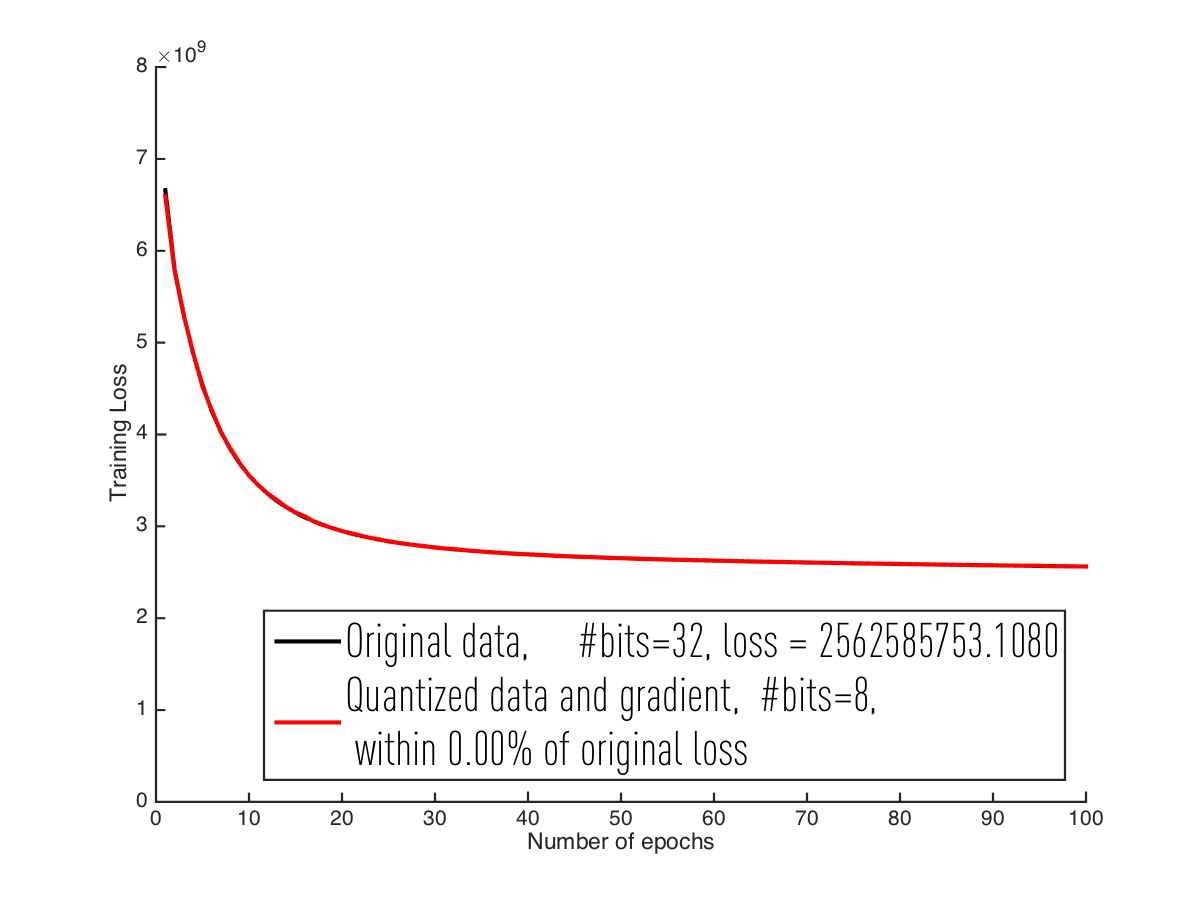
\includegraphics[width=\columnwidth]{lr/real/cadata/8dg01}
    \caption{Quantized data and gradient, initial stepsize = 0.1, 8-bit quantization}
    \end{subfigure}
    \begin{subfigure}[h]{.3\columnwidth}
    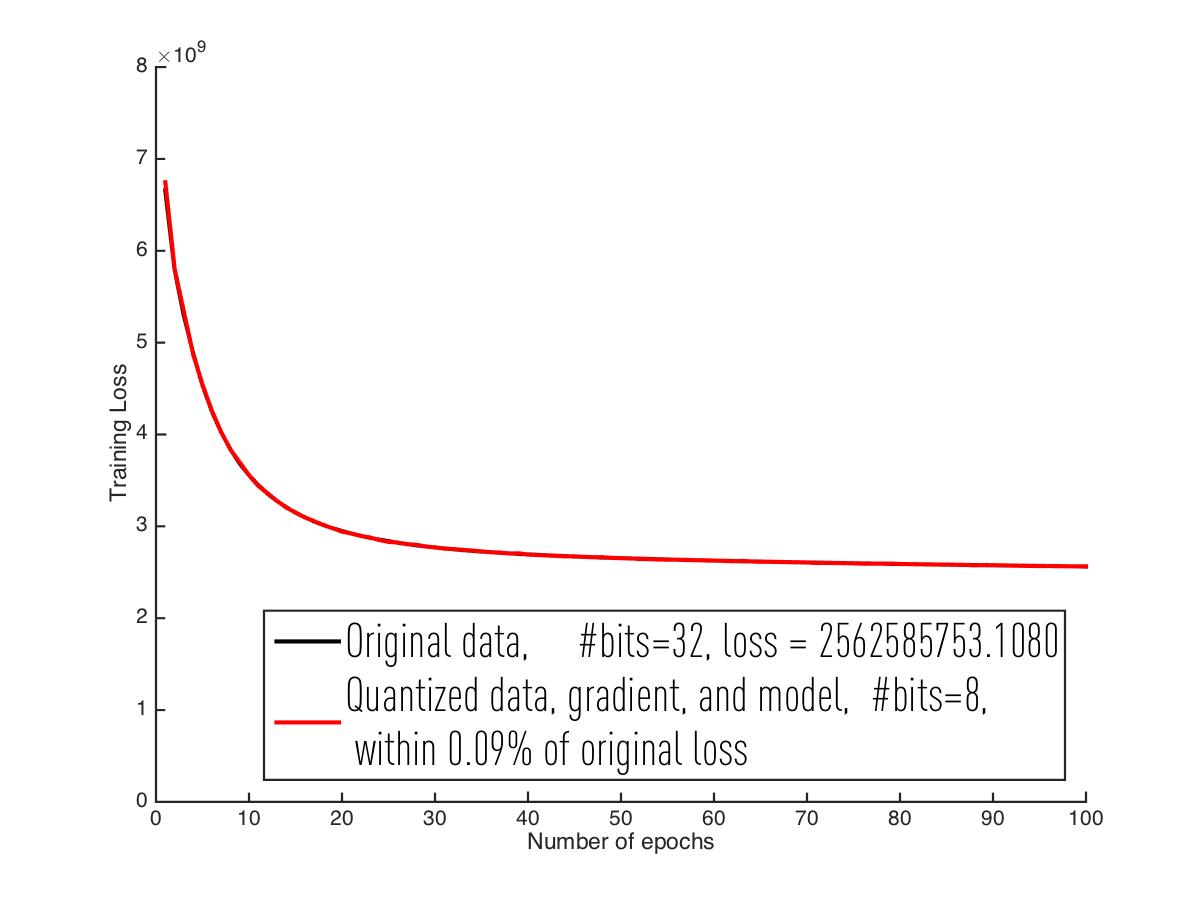
\includegraphics[width=\columnwidth]{lr/real/cadata/8dgm01}
     \caption{Quantized data, gradient, and model, initial stepsize = 0.1, 8-bit quantization}
    \end{subfigure}
    
\caption{ZipML on Linear Regression using \texttt{cadata} dataset. 3-bit version is good enough to get a comparable empirical convergence rate to the same loss; with 8-bit we get almost the same result as the original 32-bit data}
\label{fig:lrcadata}
\end{figure}



\subsection{Least Squares Support Vector Machines}

We now validate ZipML for least squares SVM.
We present the results for \texttt{cod-rna} in Figure~\ref{fig:lssvmcodrna}, the result for \texttt{covtype} in Figure~\ref{fig:lssvmcovtype}, and the result for \texttt{ijcnn} in Figure~\ref{fig:lssvmijcnn},

Figures~\ref{fig:lssvmcodrna}-\ref{fig:lssvmijcnn} illustrate that for all datasets we choose and all stepsizes we run, our quantization framework
converges to the same solution with comparable
empirical convergence rate and that 3-bit quantization is sufficient to achieve that.


\begin{figure}[h]
\centering
    \begin{subfigure}[h]{.3\columnwidth}
    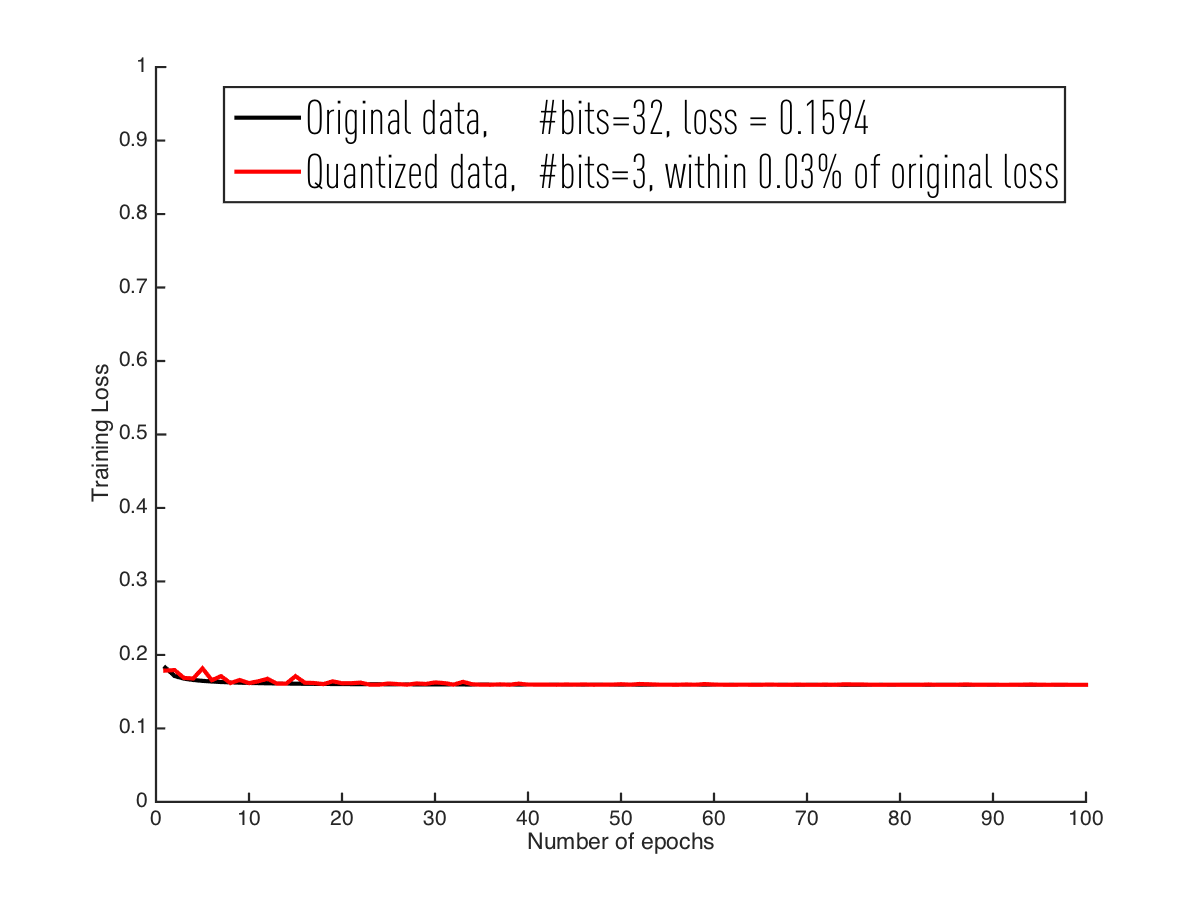
\includegraphics[width=\columnwidth]{lssvm/cod-rna/d001}
    \caption{Quantized data, initial stepsize = 0.01}
    \end{subfigure}
    \begin{subfigure}[h]{.3\columnwidth}
    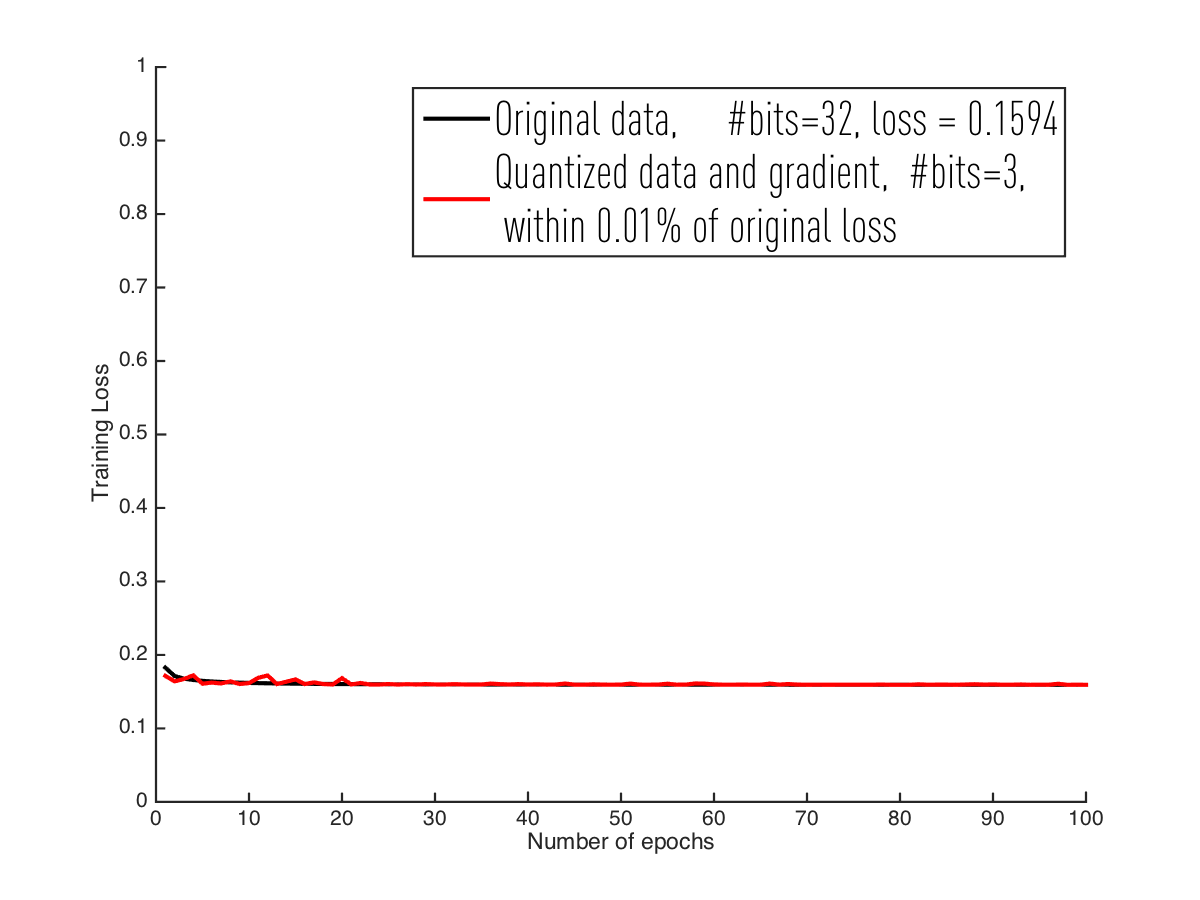
\includegraphics[width=\columnwidth]{lssvm/cod-rna/dg001}
    \caption{Quantized data and gradient, initial stepsize = 0.01}
    \end{subfigure}
    \begin{subfigure}[h]{.3\columnwidth}
    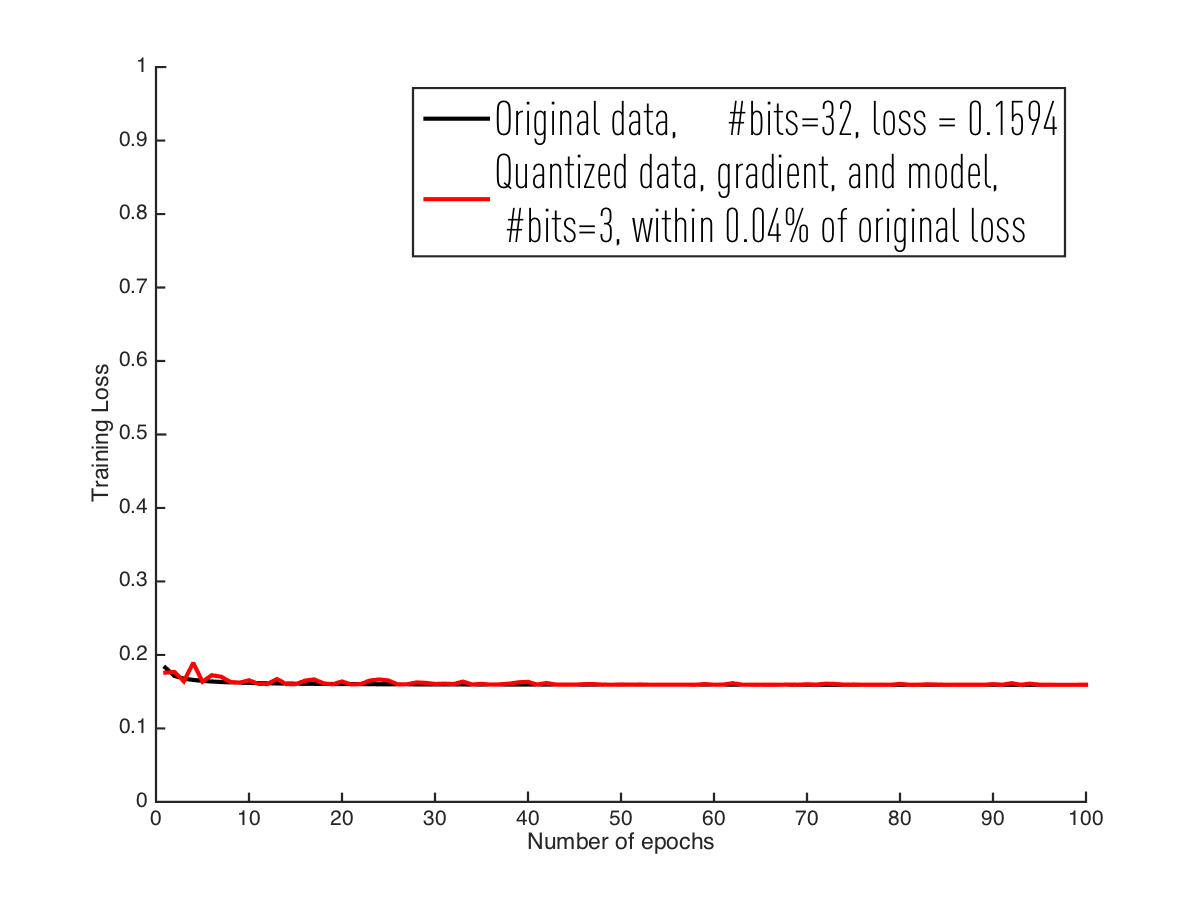
\includegraphics[width=\columnwidth]{lssvm/cod-rna/dgm001}
     \caption{Quantized data, gradient, and model, initial stepsize = 0.01}
    \end{subfigure}
    
\caption{ZipML on LSSVM using \texttt{cod-rna} dataset}
\label{fig:lssvmcodrna}
\end{figure}

\begin{figure}[h]
\centering
    \begin{subfigure}[h]{.3\columnwidth}
    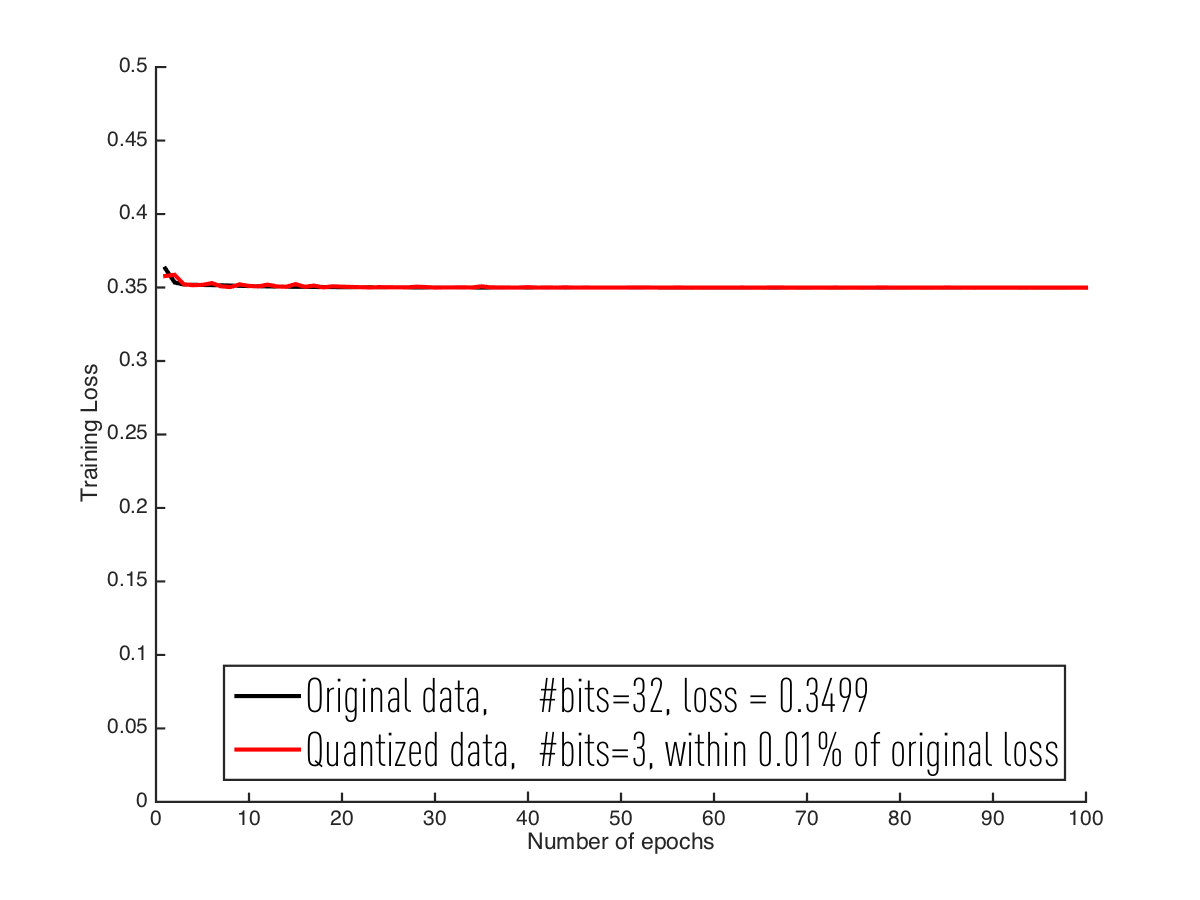
\includegraphics[width=\columnwidth]{lssvm/cov-type/d001}
    \caption{Quantized data, initial stepsize = 0.01}
    \end{subfigure}
    \begin{subfigure}[h]{.3\columnwidth}
    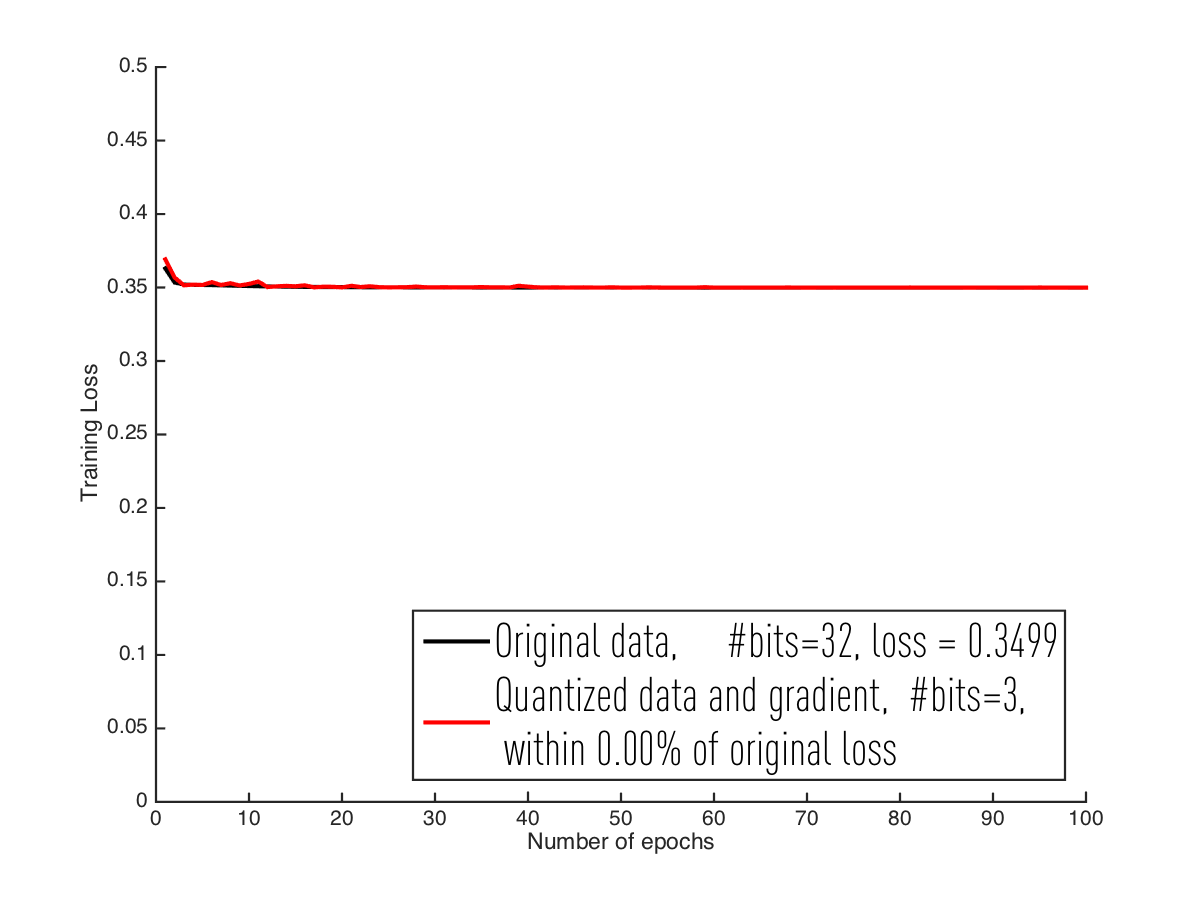
\includegraphics[width=\columnwidth]{lssvm/cov-type/dg001}
    \caption{Quantized data and gradient, initial stepsize = 0.01}
    \end{subfigure}
    \begin{subfigure}[h]{.3\columnwidth}
    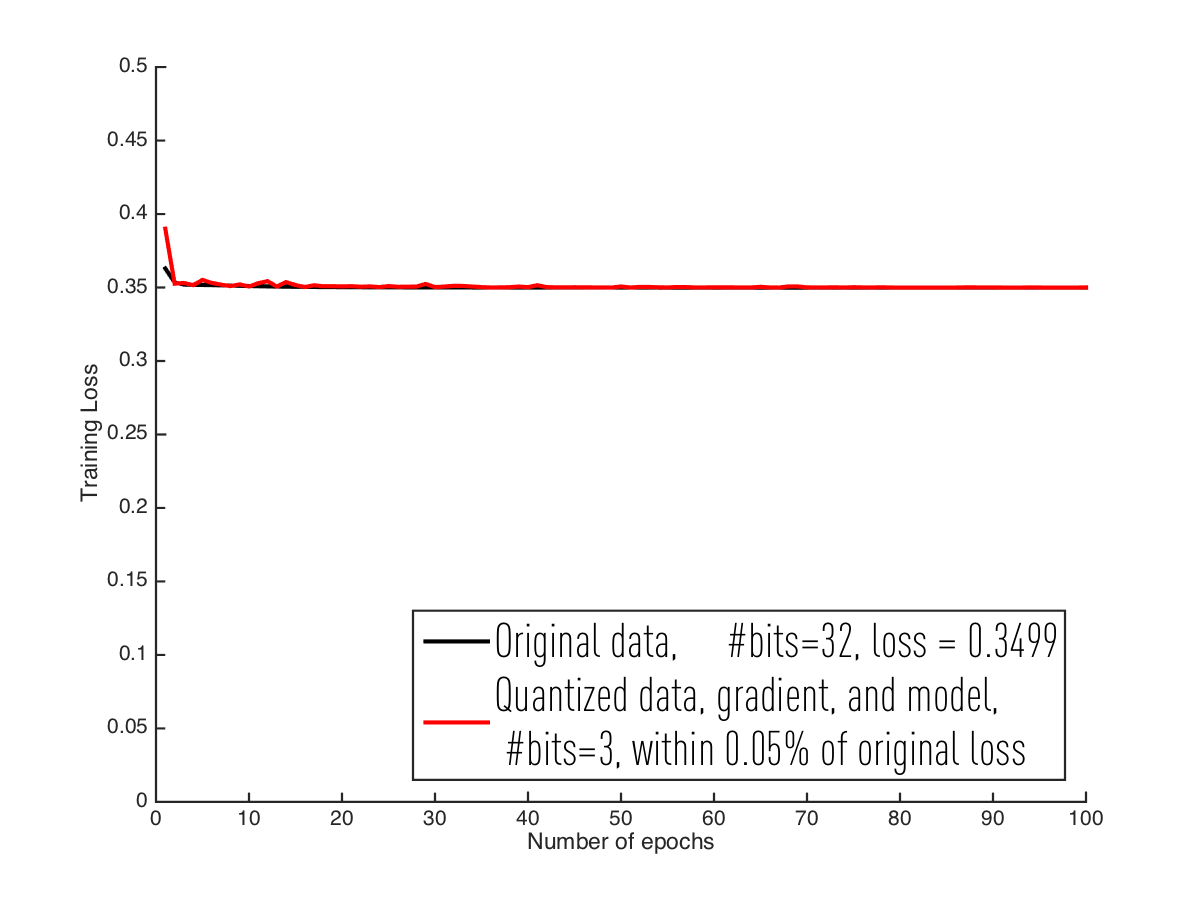
\includegraphics[width=\columnwidth]{lssvm/cov-type/dgm001}
     \caption{Quantized data, gradient, and model, initial stepsize = 0.01}
    \end{subfigure}
    
\caption{ZipML on LSSVM using \texttt{covtype} dataset}
\label{fig:lssvmcovtype}
\end{figure}



\begin{figure}[h]
\centering
    \begin{subfigure}[h]{.3\columnwidth}
    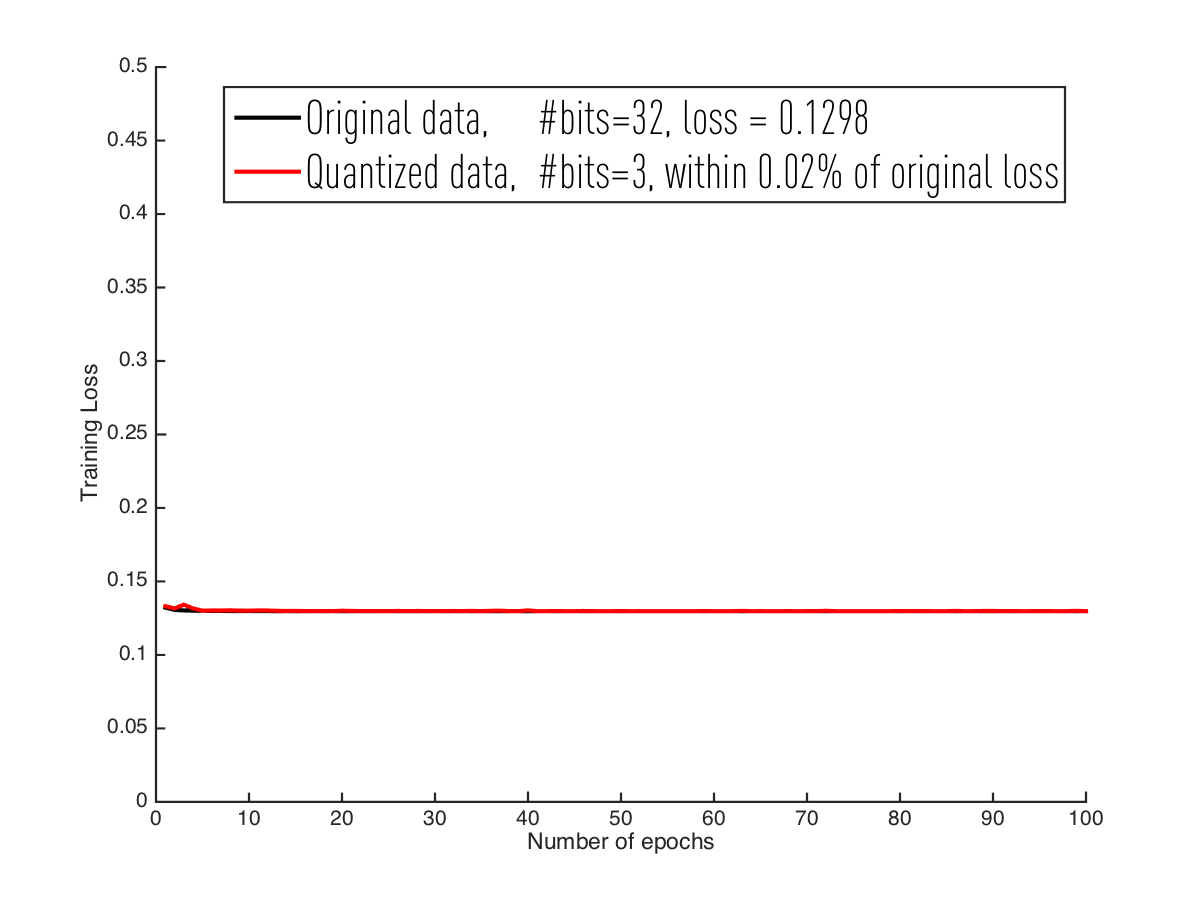
\includegraphics[width=\columnwidth]{lssvm/ijcnn/d001}
    \caption{Quantized data, initial stepsize = 0.01}
    \end{subfigure}
    \begin{subfigure}[h]{.3\columnwidth}
    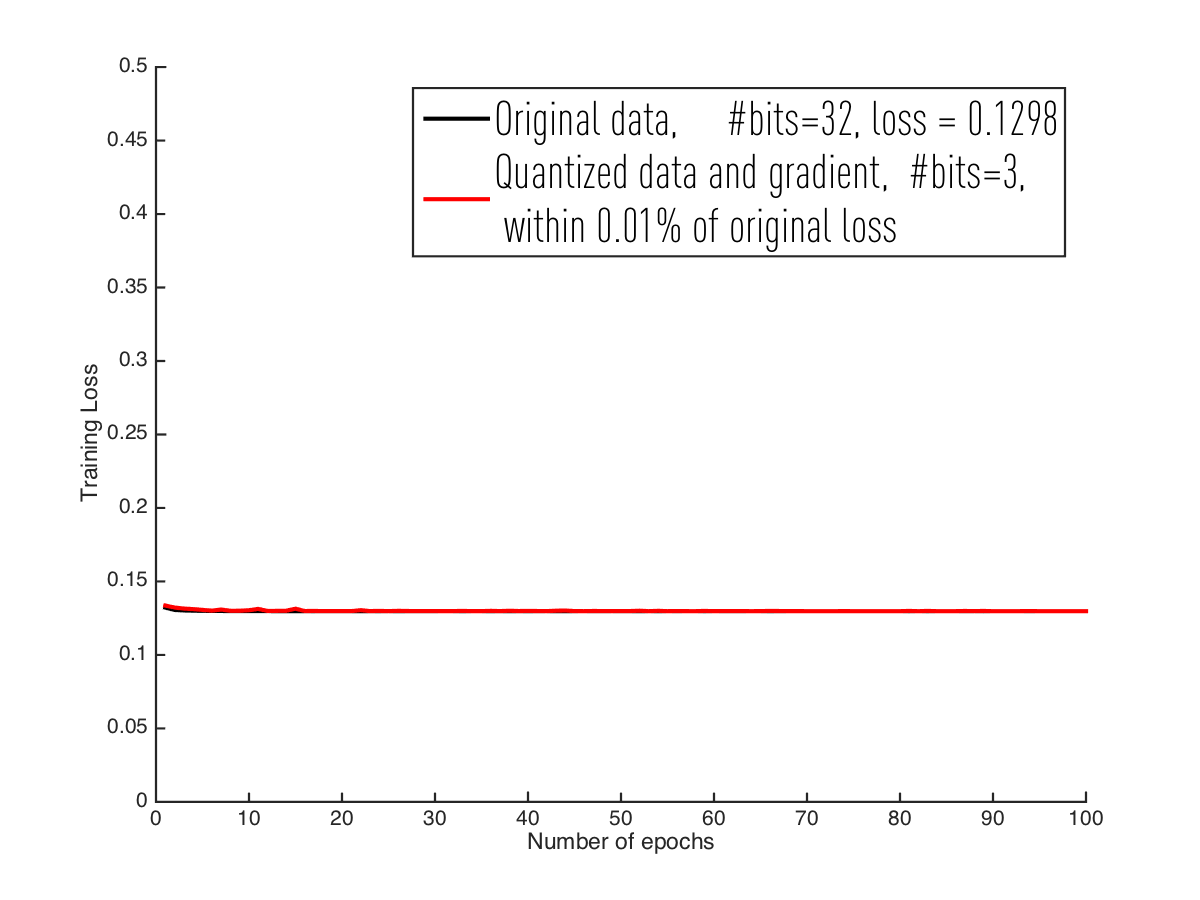
\includegraphics[width=\columnwidth]{lssvm/ijcnn/dg001}
    \caption{Quantized data and gradient, initial stepsize = 0.01}
    \end{subfigure}
    \begin{subfigure}[h]{.3\columnwidth}
    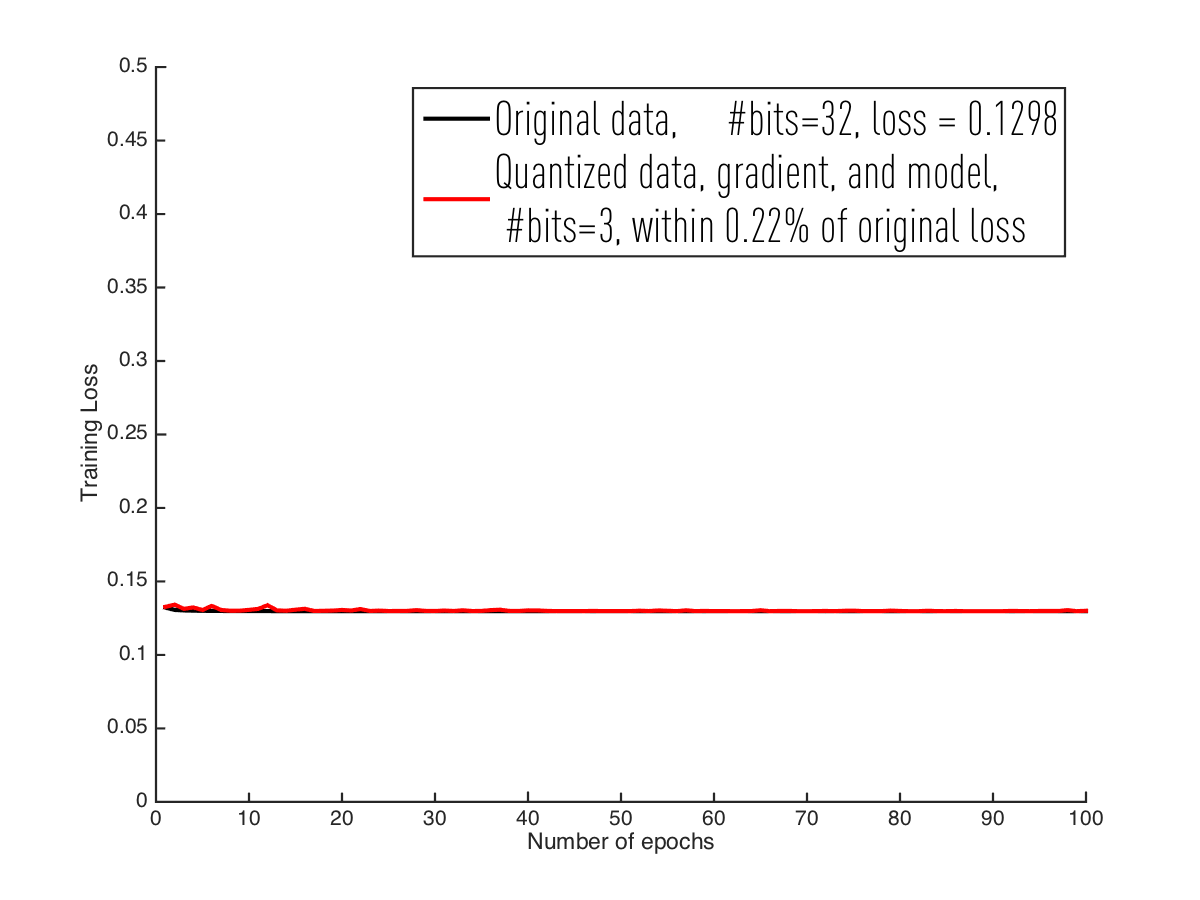
\includegraphics[width=\columnwidth]{lssvm/ijcnn/dgm001}
     \caption{Quantized data, gradient, and model, initial stepsize = 0.01}
    \end{subfigure}
    
\caption{ZipML on LSSVM using \texttt{ijcnn} dataset}
\label{fig:lssvmijcnn}
\end{figure}



\subsection{Support Vector Machines}
\label{sec:svm}

Finally we validate ZipML in the context of support vector machines (SVM).

Our experimental results for SVM are given in Figure~\ref{fig:svm}. For all datasets and stepsizes we chose, 8-bit quantization was good enough to converge to the same solution with using original data. By using importance sampling, we only need to fetch 32-bit orginal data 2\% to 7\% times. This will add an overhead of at most 2.34 bits on average for each sample we quantize, meaning that each sample we quantize is on average about 10-bit. We get comparable results to running SVM with original data, while using 3 times less memory.%\todo{Over what?}

\begin{figure}[h]
\centering
    \begin{subfigure}[b]{.3\columnwidth}
    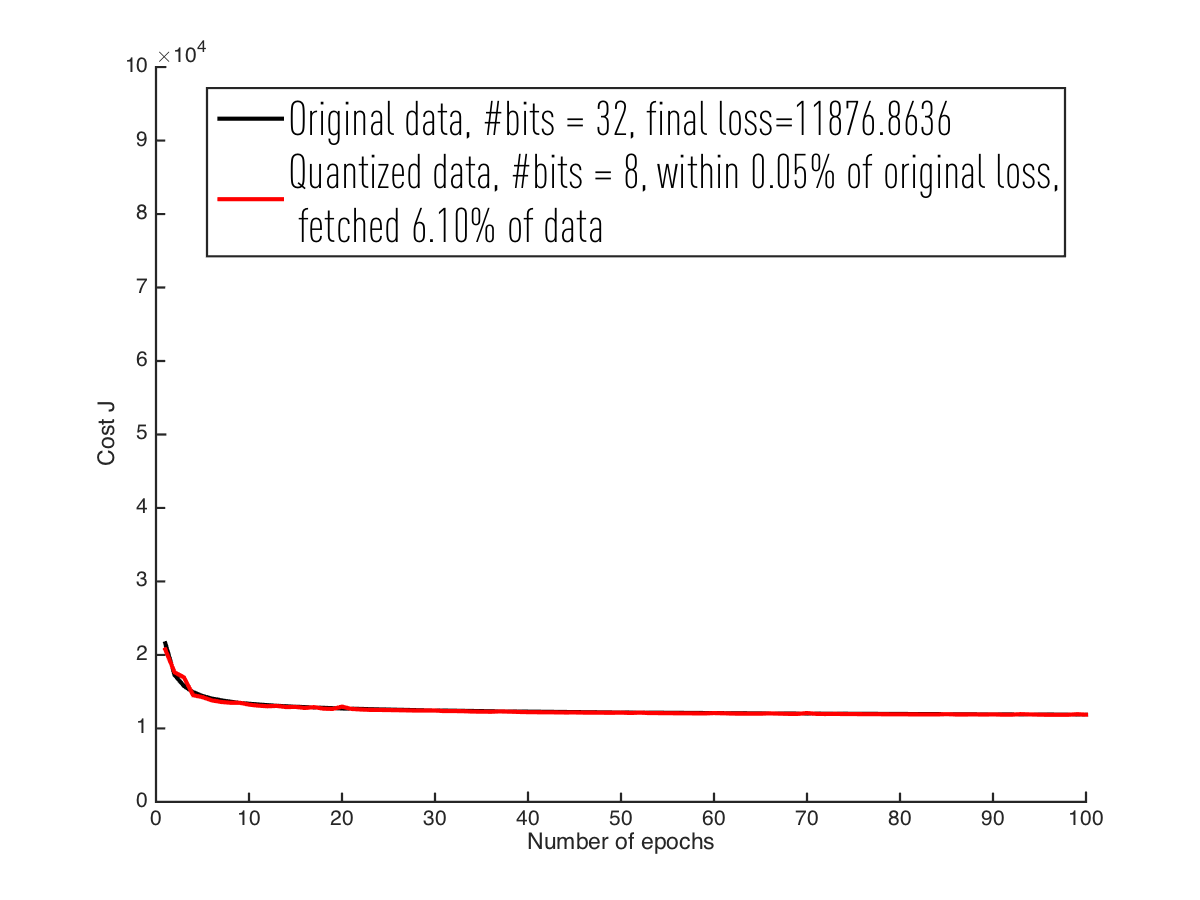
\includegraphics[width=\columnwidth]{svm/cod-rna/001}
    \caption{\texttt{cod-rna} dataset, initial stepsize = 0.01}
    \end{subfigure}
    \begin{subfigure}[b]{.3\columnwidth}
    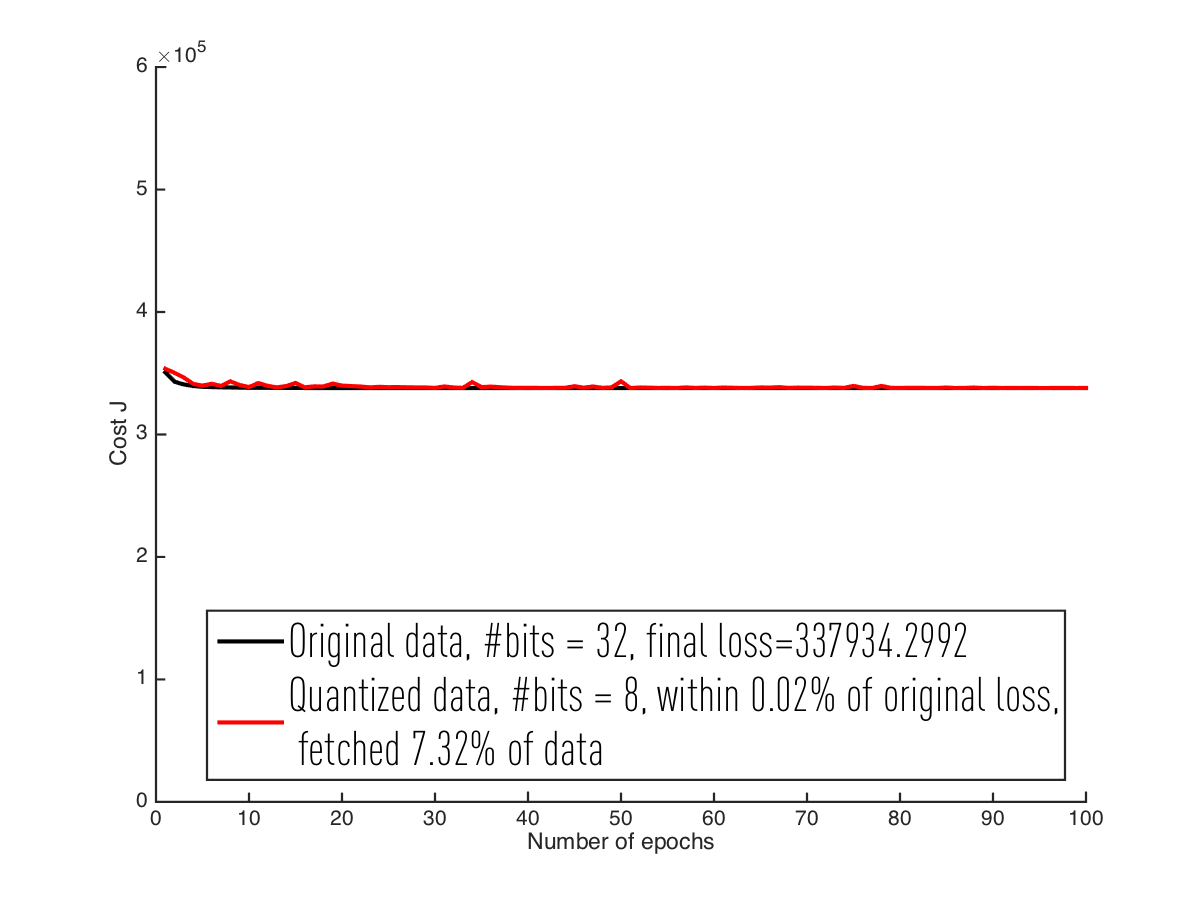
\includegraphics[width=\columnwidth]{svm/cov-type/001}
    \caption{\texttt{covtype} dataset, initial stepsize = 0.01}
    \end{subfigure}
    \begin{subfigure}[b]{.3\columnwidth}
    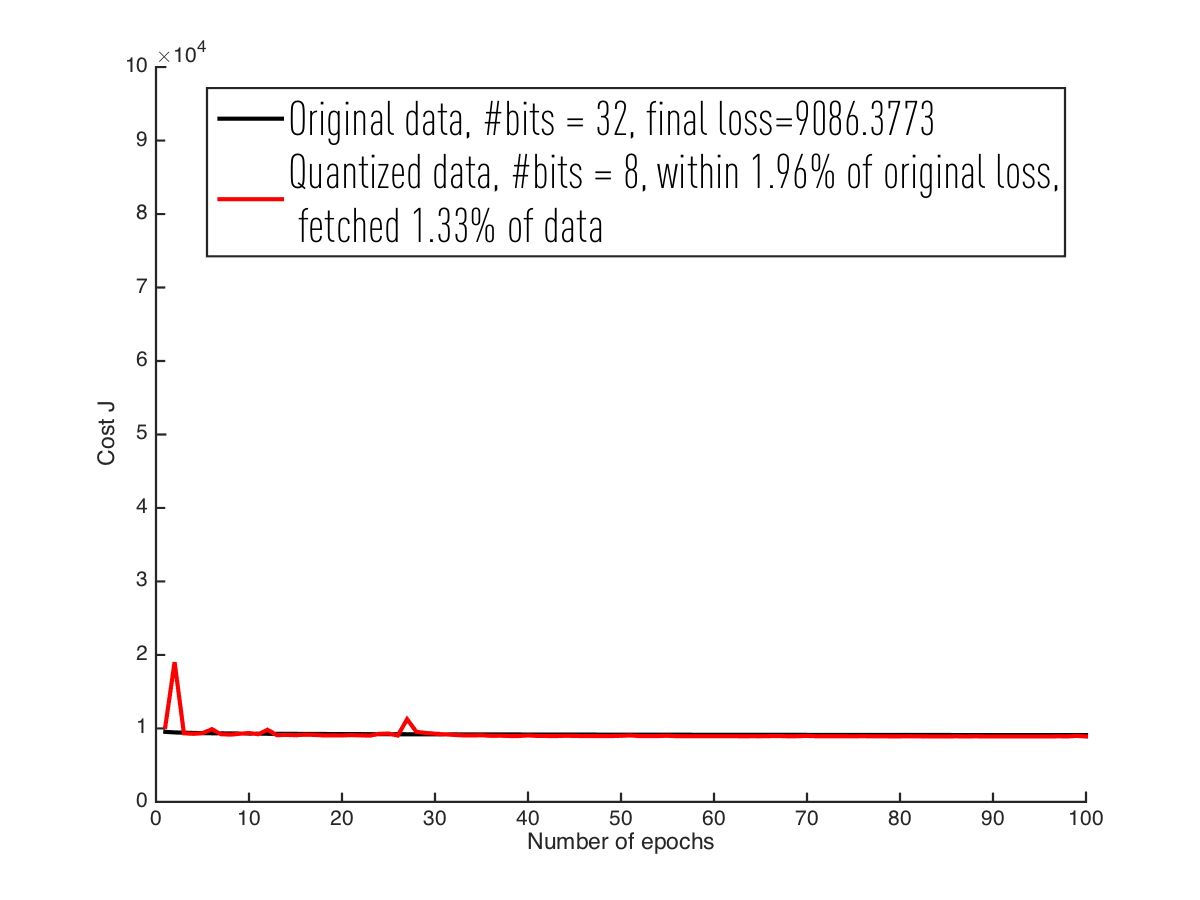
\includegraphics[width=\columnwidth]{svm/ijcnn/001}
    \caption{\texttt{ijcnn} dataset, initial stepsize = 0.01}
    \end{subfigure}
\caption{ZipML on SVM using 8-bit quantization for various datasets}
\label{fig:svm}
\end{figure}





\section{Ongoing Efforts}

%\subsection{Systems}
%
%The end-to-end low-precision representation of ZipML
%provides a range of opportunities related to system
%research. We are currently actively working
%on several system projects enabled by ZipML
%and we describe them briefly.
%
%
%\todo{Dan: How about networks? They're not really theory :) }
%
%\begin{enumerate}
%\item {\bf Hardware Primitives and Near-memory Computation.}
%ZipML's stochastic rounding scheme means that the rounding
%result for different epochs are likely to be different. In
%this scenario, an open system question is where the stochastic
%rounding procedure happens--If everytime that rounding 
%happens one need to transfer the original data from 
%memory to CPU, we do not get much benefit by using ZipML.
%Therefore, one of our ongoing projects is to design hardware primitives
%for stochastic rounding and pushes these computations
%to storage devices such as SSD and DRAM. 
%
%\item {\bf ``Machine Learning Index'' for In-Database Analytics.}
%In-Database analytics systems support training of machine
%learning models over relations (tables) stored inside 
%a relational database system (RDBMS). In RDBMS, users
%can create index such as B-Tree or hash index to speed
%up SQL queries. ZipML provides a novel way to construct
%index for ``machine learning queries'' by pre-materialize
%a set of samples and store them on disk. One of
%our ongoing projects is to understand the possibility of
%integrating this novel index into existing in-database analytics 
%systems such as Pivotal MADlib or SAP HANA PAL.
%
%\item {\bf ``Progressive Analytics''} We believe that
%ZipML provides a theoretically sound way to ``rapidly prototype''
%a machine learning model by training over low-precision
%data. One of our ongoing projects is to define and implement
%a {\em realtime}, {\em progressive}, analytics systems--Given
%10GB data, the users get a ``good enough'' model within 100ms
%to continue his follow up tasks while this model keeps
%getting refined (similar to how progressive JPEG works).
%In this way, the user does not have the feeling of waiting
%for machine learning and analytics to finish, and we believe
%this could enable a new interaction model between users and
%analytics systems.
%
%\item {\bf Edge Computing and Embedded Systems.} Many sensor
%networks in industrial environments suffer from the limitation
%of data transformation (due to power, price, and physical 
%locations). With our industrial partners, one of our
%ongoing projects is to integrate ZipML into embedded 
%systems to enable more effective data transformation 
%over sensor networks when a joint machine learning model 
%needs to be trained.
%
%\item {\bf ``Warm Storage'' Machine Learning.} Data
%involved in training a model learning model are
%often ``hot data''--they need to be put in fast storage
%such as DRAM. However, on machines whose memory bandwidth 
%is only one order
%of magnitude faster than disk bandwidth, with ZipML
%we expect to
%observe the training time to be similar no matter
%the data is on disk or in memory. We empirically validated
%this on  EC2 \texttt{c4.8xlarge} instance. This
%implies that the operating cost of machine learning
%cloud services such as Azure could be significantly
%lowered by storing more data onto cheaper/colder 
%secondary  storages without the users observe much slowdown
%or any difference in training quality. Similarly,
%users can also choose to use cheaper slower storage 
%to replace the more expensive ones. One of our
%ongoing projects is to integrate ZipML to
%machine learning cloud services and understand
%its system implications.
%
%\end{enumerate}




%\subsection{Theory}

\begin{itemize}
	\item {\bf General Loss Functions.} 
	A key question in the context of our work is whether it is possible to perform sample and model quantization 
	in the context of more complex loss functions, such as hinge loss, sigmoid, logit, or rectified linear units. 
	We speculate that this might be possible by adapting the alternating direction method of multipliers (ADMM)~\cite{ADMM}, 
	or via error correction.  
	
	\item {\bf SVM with Corrupted Labels.}  
	The discussion in Section~\ref{sec:svm} suggests the following general question: 
	Does stochastic gradient descent provide any convergence guarantees if a subset of the samples considered in an iteration (the ones with low margin) have flipped labels?
	
	\item {\bf Better Coding.}  
	We currently only employ simple coding techniques. However, it is interesting to consider whether \emph{difference coding} can be employed to code the difference between two consecutive gradients, or to reduce the bandwidth overhead of double sampling.  

\iffalse
    \item {\bf Quantized Activations and Model Compression.}  
	It is also interesting to consider whether accuracy (test loss) can be preserved when the model is quantized. 
	This question is especially important in the context of \emph{model compression}, which is an active area of research.\footnote{https://petewarden.com/2016/05/03/how-to-quantize-neural-networks-with-tensorflow/}
\fi

    \item {\bf Compression/Variance Tradeoffs.} It is not clear that the trade-offs between bit width and variance increase are tight, and we currently do not analyze the dependence on the condition number of the dataset. 
    
    \item {\bf Alternative Quantizations.} The current quantization strategy is to equally partition the interval $[0, 1]$. 
    We plan to investigate whether heterogeneous intervals can reduce variance.
    
    
    
\end{itemize}


\fi


\end{document}
